\chapter{Vector Spaces and Coordinate Bases}
\label{chap:vec_space}

The previous chapters have provided a basic understanding of matrices and vectors separately. What bridge these two quantities together are the concepts of \textit{vector (sub)spaces}, \textit{linear combination}, \textit{span}, \textit{linear independence}. With all of these, we can revisit the process of Gaussian Elimination from the view of \textit{column-row factorization}. Then, we will learn how to find \textit{coordinate bases} for vector spaces so as to represent vectors in different coordinate systems. Finally, we are going to investigate about the so-called \textit{four fundamental subspaces} induced by a matrix and see how they are interconnected via the \textit{Rank-Nullity Theorem}.

\section{Making of the Real $n$-space $\mathbb{R}^n$}

\subsection{$\mathbb{R}^n$ as a Vector Space}

We have briefly mentioned in Definition \ref{defn:real_nspace} that the real $n$-space $\mathbb{R}^n$ is mathematically a vector space, but without stating the actual requirements. In fact, to be qualified as a \index{Vector Space}\keywordhl{vector space}, a set has to satisfy the ten axioms below. We will limit ourselves to \index{Vector Space!Real Vector Space}\keywordhl{real vector spaces} for now.
\begin{defn}[Axioms of a (Real) Vector Space]
\label{defn:realvecspaceaxiom}
A \textit{real} vector space is a non-empty set $\mathcal{V}$ with the zero vector \textbf{0}, such that for all elements (vectors) $\vec{u}, \vec{v}, \vec{w} \in \mathcal{V}$ in the set, and \textit{real} numbers (as the \textit{scalars}) $a, b \in \mathbb{R}$ (for a complex vector space replace $\mathbb{R}$ by $\mathbb{C}$ here), we have
\begin{enumerate}
\item $\vec{u} + \vec{v} \in \mathcal{V}$ (Closure under Vector Addition: Addition between two vectors is defined and the resulting vector is still in the vector space.)
\item $\vec{u} + \vec{v} = \vec{v} + \vec{u}$ (Commutative Property of Addition)
\item $(\vec{u} + \vec{v}) + \vec{w} = \vec{u} + (\vec{v} + \vec{w})$ (Associative Property of Addition)
\item $\vec{u} + \textbf{0} = \textbf{0} + \vec{u} = \vec{u}$ (Zero Vector as the Additive Identity)
\item For any $\vec{u}$, there exists $\vec{w}$ such that $\vec{u} + \vec{w} = \textbf{0}$. This $\vec{w}$ is denoted as $-\vec{u}$. (Existence of Additive Inverse)
\item $a\vec{u} \in \mathcal{V}$ (Closure under Scalar Multiplication: Multiplying a vector by any scalar (a real/complex number for a real/complex vector space) is defined and the resulting vector is still in the vector space.)
\item $a(\vec{u} + \vec{v}) = a\vec{u} + a\vec{v}$ (Distributive Property of Scalar Multiplication)
\item $(a+b)\vec{u} = a\vec{u} + b\vec{u}$ (Distributive Property of Scalar Multiplication)
\item $a(b\vec{u}) = (ab)\vec{u}$ (Associative Property of Scalar Multiplication)
\item $1\vec{u} = \vec{u}$ (The real number $1$ as the Multiplicative Identity)
\end{enumerate}
\end{defn}
The real $n$-space $\mathbb{R}^n$ satisfies all the axioms above and is finite-dimensional, particularly $n$-dimensional (the notion of dimension here should be intuitive, but we will go through it more precisely later), with addition and scalar multiplication being the usual ones as defined in Section \ref{section:vectoraddmul}, and the zero vector is simply $\textbf{0} = (0,0,0,\ldots,0)^T$ with $n$ zeros. We will not do it here but interested readers can try to justify all of them. To build the definition of a vector space from these axioms allows the generalization and application of its utilities to other sets that share the same abstract structure. \textcolor{red}{However, for most usages, we will focus on $\mathbb{R}^n$\footnote{We actually have a very good reason to do so, as we will see in the next chapter: any $n$-dimensional real vector space is \textit{isomorphic} to and can be treated like $\mathbb{R}^n$.}, and the vector space axioms are provided above mainly for reference.} We defer the treatment of complex vector spaces to Chapter \ref{chap:complex}.

\subsection{Subspaces of $\mathbb{R}^n$}
\label{section:Rnsubspace}

It will be very boring if we consider only the whole $\mathbb{R}^n$ as a vector space. In last chapter, we show that geometrically there can be lower-dimensional shapes like lines/planes/hyperplanes residing in $\mathbb{R}^n$. This raises the question if we can similarly find \index{Subspace}\keywordhl{subspaces} embedded in $\mathbb{R}^n$ that is a subset of $\mathbb{R}^n$ which still fulfills the aforementioned vector space axioms such that it is a vector space in its own right. Nevertheless, to determine if a subset of vector space is a subspace, we don't need to check all the ten axioms but rather just two of them.
\begin{thm}[Criteria for a Subspace]
\label{thm:subspacecriteria}
If $\mathcal{W}$ is a non-empty subset of a (real) vector space $\mathcal{V}$ (i.e. $\mathcal{W} \subseteq \mathcal{V}$), then $\mathcal{W}$ is called a (real) subspace of $\mathcal{V}$ if the following criteria are satisfied:
\begin{enumerate}
\item For any $\vec{u}, \vec{v} \in \mathcal{W}$, $\vec{u} + \vec{v} \in \mathcal{W}$ (Closed under Addition)
\item For any scalar $a$ ($\in \mathbb{R}$) and $\vec{u} \in \mathcal{W}$, $a\vec{u} \in \mathcal{W}$ (Closed under Scalar Multiplication), particularly when $a = 0$, $0\vec{u} = \textbf{0} \in \mathcal{W}$ so that a subspace always contains the zero vector of $\mathcal{V}$.
\end{enumerate}
These are the same requirements of (1) and (6) in Definition \ref{defn:realvecspaceaxiom}. An equivalent condition is that, for any $\vec{u}, \vec{v} \in \mathcal{W}$ and two scalars $a$ and $b$, $a\vec{u} + b\vec{v} \in \mathcal{W}$.
\end{thm}
\begin{exmp}
Consider the following subsets of $\mathbb{R}^2$ and decide if they are subspaces of $\mathbb{R}^2$ by verifying the two criteria listed in Theorem \ref{thm:subspacecriteria}.
\begin{enumerate}[label=(\alph*)]
\item The line $x - 2y = 0$,
\item The $y$-axis,
\item The positive $y$-axis,
\item The line $2x + y = 1$,
\item The parabola $y = x^2$,
\item The point $(-1,1)^T$,
\item The first quadrant $x > 0$, $y > 0$,
\item The origin $\textbf{0} = (0,0)^T$,
\item $\mathbb{R}^2$ itself.
\end{enumerate}
\end{exmp}
\begin{solution}
\begin{enumerate}[label=(\alph*)]
\item The vector form of the line is $\mathcal{W} = \{(x,y)^T = t(2,1)^T \mid -\infty < t < \infty\}$. To check the first condition, let's say $\vec{u} = t_1(2,1)^T \in \mathcal{W}$ and $\vec{v} = t_2(2,1)^T \in \mathcal{W}$ are vectors in $\mathcal{W}$ for some $t_1$ and $t_2$, then $\vec{u} + \vec{v} = t_1(2,1)^T + t_2(2,1)^T = (t_1 + t_2)(2,1)^T = s(2,1)^T \in \mathcal{W}$ where $s = t_1 + t_2$ also lies on the same straight line of $x-2y = 0$ and is another vector in $\mathcal{W}$, so $\mathcal{W}$ is closed under addition. To check the second condition, this time we simply let $\vec{u} = t(2,1)^T \in \mathcal{W}$. Subsequently, $a\vec{u} = at(2,1)^T = r(2,1)^T \in \mathcal{W}$, for any scalar $a$ and $r = at$, so it is also closed under scalar multiplication. Hence the line $x-2y = 0$ is a subspace of $\mathbb{R}^2$.
\item Same arguments as above but with $\mathcal{W} = \{(x,y)^T = t(0,1)^T \mid -\infty < t < \infty\}$, so the $y$-axis is also a subspace of $\mathbb{R}^2$.
\item For any point on the positive $y$-axis, multiplying it by a negative number places it on the negative $y$-axis instead, so it is not closed under scalar multiplication and thus not a subspace of $\mathbb{R}^2$. 
\item Denote the collection of points on the line as $\mathcal{W}$. Pick $\vec{u} = (1, -1)^T \in \mathcal{W}$ and $\vec{v} = (0, 1)^T \in \mathcal{W}$, then $\vec{u} + \vec{v} = (1, 0)^T \notin \mathcal{W}$ as $2(1) + (0) = 2 \neq 1$, so it is not closed under addition and fails to be a subspace of $\mathbb{R}^2$.
\item Denote the collection of points on the parabola as $\mathcal{W}$. Pick $\vec{u} = (1,1)^T \in \mathcal{W}$ and $\vec{v} = (2,4)^T \in \mathcal{W}$, then $\vec{u} + \vec{v} = (3,5)^T \notin \mathcal{W}$ is apparently not on the parabola, so it is not closed under addition and can't be a subspace of $\mathbb{R}^2$.
\item It is easy to see that it fails to be closed under either addition or scalar multiplication (for example, take $a(-1,1)^T$ with $a\neq 1$) and is not a subspace of $\mathbb{R}^2$.
\item Denote the collection of points on the first quadrant as $\mathcal{W}$. Pick $\vec{u} = (1,1)^T \in \mathcal{W}$ (or any other point), then multiplying it by $-1$ will produce $(-1)\vec{u} = -(1,1)^T = (-1,-1)^T \notin \mathcal{W}$ which is outside the first quadrant. Therefore, it is not closed under scalar multiplication and hence not a subspace of $\mathbb{R}^2$.
\item It trivially satisfies the two criteria ($\textbf{0}$ is the only element in the set, $\textbf{0} + \textbf{0} = \textbf{0}$ and $a\textbf{0} = \textbf{0}$ for any scalar $a$) and is a subspace of $\mathbb{R}^2$.
\item $\mathbb{R}^2$ is a vector space to begin with and technically a subset of itself (it trivially contains itself) so by definition it is a subspace of $\mathbb{R}^2$.
\end{enumerate}
\end{solution}
Generalizing the above discussion, we can easily infer that for $\mathbb{R}^2$, only the origin (the zero subspace), an infinitely long straight line that passes through the origin, or $\mathbb{R}^2$ itself can be its subspaces (see the schematic in Figure \ref{fig:R2subspace}). We often use the phrase \index{Subspace!Proper Subspace}\keywordhl{proper subspaces} to exclude the accommodating vector space itself ($\mathbb{R}^2$ in this case). For any $\mathbb{R}^n$, the \index{Subspace!Zero Subspace}\keywordhl{zero subspace} $\{\textbf{0}\}$ and \index{Subspace!Improper Subspace}\keywordhl{improper subspace} $\mathbb{R}^n$ are always two subspaces of it. 
\begin{figure}
    \centering
    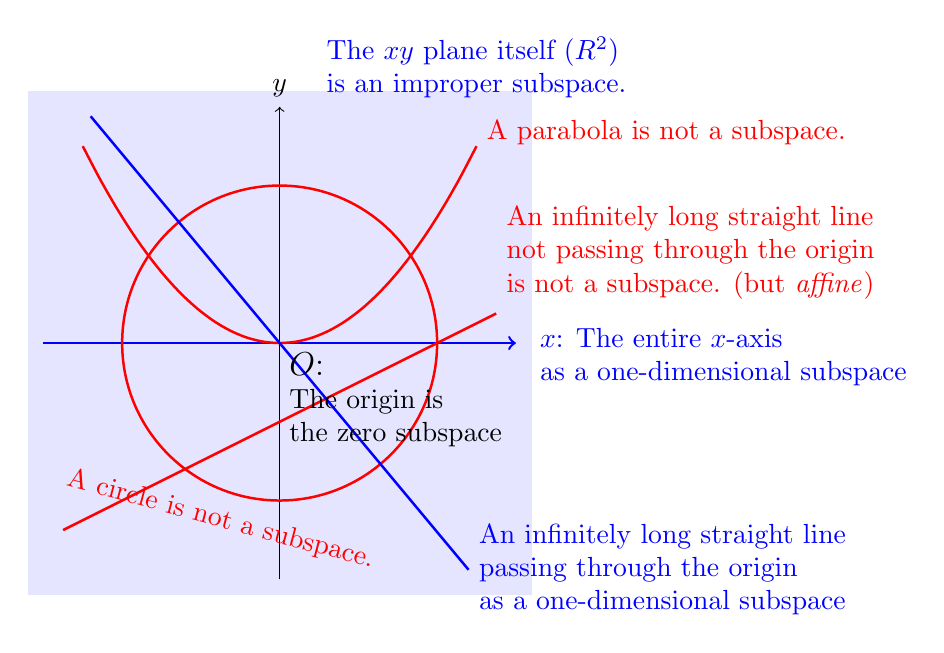
\begin{tikzpicture}
    \filldraw[draw=none, fill=blue, opacity=0.1]
    (-3.2,3.2) -- (3.2,3.2) -- (3.2,-3.2) -- (-3.2,-3.2) -- cycle;
    \draw[blue, line width = 0.9, ->] (-3,0)--(3,0) node[right, align=left, xshift=5, yshift=-5]{$x$: The entire $x$-axis \\
    as a one-dimensional subspace};
    \draw[->] (0,-3)--(0,3) node[above]{$y$}; 
    \draw[red, line width = 0.9] circle (2);
    \node[blue, align=left, anchor=center] at (2.5, 3.5) {The $xy$ plane itself ($\mathbb{R}^2$) \\ is an improper subspace.};
    \draw[red, line width = 0.9] plot[smooth, domain=-2.5:2.5] (\x, 0.4 * \x * \x) node[right, align=left, yshift=5]{A parabola is not a subspace.};
    \draw[red, line width = 0.9] plot[smooth, domain=-2.75:2.75] (\x, 0.5* \x -1) node[right, align=left, yshift=22]{An infinitely long straight line \\
    not passing through the origin \\
    is not a subspace. (but \textit{affine})};
    \draw[blue, line width = 0.9] plot[smooth, domain=-2.4:2.4] (\x, -1.2 * \x) node[right, align=left]{An infinitely long straight line \\passing through the origin \\as a one-dimensional subspace};
    \node[red,rotate=-15] at (-0.75, -2.25) {A circle is not a subspace.};
    \node[align=left, anchor=north west]{\large $O$: \\ The origin is\\ the zero subspace};
    \end{tikzpicture}
    \caption{Some examples (blue) and non-examples (red) of subspaces in $\mathbb{R}^2$.}
    \label{fig:R2subspace}
\end{figure}\par
Short Exercise: Determine if the following subsets of $\mathbb{R}^3$ is a subspace of $\mathbb{R}^3$.\footnote{Yes, No, Yes, No, Yes, No, Yes, No, No. In fact, all possible subspaces of $\mathbb{R}^3$ are $\{\textbf{0}\}$, any infinitely long line/extending plane through the origin and $\mathbb{R}^3$ itself.}
\begin{enumerate}[label=(\alph*)]
\item The origin $\textbf{0} = (0,0,0)^T$,
\item The point $(1,2,3)^T$,
\item The line $(x,y,z)^T = t(-1, 1, 2)^T$ for any scalar $t$,
\item The line $(x,y,z)^T = (1, -1, 3) + t(1, 2, -1)^T$ for any scalar $t$,
\item The plane $x + 2y - 3z = 0$,
\item The plane $x + y + 4z = 5$,
\item $\mathbb{R}^3$ itself,
\item The sphere $x^2 + y^2 + z^2 = 1$,
\item The cone $x^2 + y^2 = z^2$.
\end{enumerate}
Further generalization motivated by the short exercise above leads to an intuitive result that, for $\mathbb{R}^n$, all its possible subspaces are geometrically "flat shapes" that pass through the origin and extend infinitely. On the other hand, any "curved shape" will not qualify as a subspace. From now on, we assume all vector (sub)spaces mentioned are finite-dimensional (again, we will clarify this notion later) unless otherwise specified.

\subsection{Span by Linear Combinations of Vectors}
\label{section:span}
The last section sees subspaces from a top-down perspective as some subsets of a larger vector space. Here, we are going to take another look at them with a bottom-up perspective, about how to generate a subspace of $\mathbb{R}^n$ from some of its vectors. To do so, we need to first understand what is a \index{Linear Combination}\keywordhl{linear combination} of vectors.
\begin{defn}[Linear Combination of Vectors]
\label{defn:linearcomb}
A linear combination of vectors $\vec{v}^{(1)}, \vec{v}^{(2)}, \vec{v}^{(3)}, \ldots, \vec{v}^{(q)} \in \mathcal{V}$ where $\mathcal{V}$ is some vector space has the form of
\begin{align*}
\sum_{j=1}^q c_j\vec{v}^{(j)} = c_1\vec{v}^{(1)} + c_2\vec{v}^{(2)} + c_3\vec{v}^{(3)} + \cdots + c_q\vec{v}^{(q)}
\end{align*}
where the coefficients $c_j$ are some scalars (real numbers for a real vector space) and the amount of vectors $q$ has to be \textit{finite}.
\end{defn}
As a small example, if there are two vectors $\vec{u} = (1,2)^T$ and $\vec{v} = (3,4)^T \in \mathbb{R}^2$, then $\vec{h} = (5,6)^T \in \mathbb{R}^2$ can be written as a linear combination of $\vec{u}$ and $\vec{v}$ because $\vec{h} = (5,6)^T = -(1,2)^T + 2(3,4)^T = -\vec{u} + 2\vec{v}$. \\
\\
Short Exercise: If $\vec{h} = (1,4)^T$ instead, express it as a linear combination of $\vec{u}$ and $\vec{v}$.\footnote{$(1,4)^T = 4(1,2)^T - (3,4)^T$.}\par

Attentive readers may realize that the short exercise above can be considered as a task to find out the solution (if any) for the system
\begin{align*}
\begin{bmatrix}
1 & 3 \\
2 & 4 \\
\end{bmatrix}
\begin{bmatrix}
c_1 \\
c_2
\end{bmatrix} =
\begin{bmatrix}
1 \\
4
\end{bmatrix}
\end{align*}
Extending this, to decide whether a vector $\vec{h} \in \mathbb{R}^n$ can be written as the linear combination of other vectors $\vec{v}^{(j)} \in \mathbb{R}^n$, $j = 1, 2, \ldots, q$, is equivalent to determining whether the linear system $A\vec{x} = \vec{h}$ has a solution, where $A$ equals to (writing out $\vec{v}^{(j)}$ in a matrix column by column)
\begin{align*}
A = \left[\begin{array}{@{}c|c|c|c@{}}
| & | & & | \\
\vec{v}^{(1)} & \vec{v}^{(2)} & \cdots & \vec{v}^{(q)} \vspace{-4pt} \\
| & | & & |
\end{array}\right]
\end{align*}
Here, the matrix product $A\vec{x}$ is a compact way to represent a linear combination of the column vectors that have been condensed into $A$.
\begin{proper}
\label{proper:linearcombmatrix}
A linear combination $c_1\vec{v}^{(1)} + c_2\vec{v}^{(2)} + c_3\vec{v}^{(3)} + \cdots + c_q\vec{v}^{(q)}$ made up of some vectors $\vec{v}^{(1)}, \vec{v}^{(2)}, \vec{v}^{(3)}, \ldots, \vec{v}^{(q)} \in \mathbb{R}^n$ as in Definition \ref{defn:linearcomb}, can be expressed by the matrix product $A\vec{x}$, where
\begin{align*}
&A = \left[\begin{array}{@{}c|c|c|c@{}}
| & | & & | \\
\vec{v}^{(1)} & \vec{v}^{(2)} & \cdots & \vec{v}^{(q)} \vspace{-4pt} \\
| & | & & |
\end{array}\right]
&\vec{x} =
\begin{bmatrix}
c_1 \\
c_2 \\
c_3 \\
\vdots \\
c_q
\end{bmatrix}
\end{align*}
From now on, we will just simply write $A = [\vec{v}^{(1)} | \vec{v}^{(2)} | \cdots | \vec{v}^{(q)}]$ and similarly for other matrices formed by column vectors when applicable to save space.
\end{proper}
From this perspective, the first/second/last column of a matrix $A$ can be extracted by
\begin{align*}
A&
\begin{bmatrix}
1 \\
0 \\
0 \\
\vdots \\
0
\end{bmatrix}
&
A&
\begin{bmatrix}
0 \\
1 \\
0 \\
\vdots \\
0
\end{bmatrix}
&
A&
\begin{bmatrix}
0 \\
0 \\
0 \\
\vdots \\
1
\end{bmatrix}
\end{align*}
and it goes similarly for any other column. Below is a small example to demonstrate the equivalence between matrix-vector products and linear combinations.
\begin{align*}
\begin{tikzpicture}[baseline=-\the\dimexpr\fontdimen22\textfont2\relax]
\matrix(mymatrix)[matrix of math nodes, left delimiter={[}, 
right delimiter={]}, anchor=center, row sep=1pt, column sep=1pt, outer sep=-2pt, nodes={text width=12pt, align=center}, ampersand replacement=\&]
{5 \& 1 \& -1 \& 2 \\
2 \& 3 \& 0 \& 7 \\
4 \& -2 \& 3 \& 1 \\};
\draw [draw=none, fill=red!50, fill opacity=0.4] (mymatrix-1-2.north west) rectangle (mymatrix-3-2.south east);
\end{tikzpicture}
\begin{bmatrix}
0 \\
\color{red}{1} \\
0 \\
0
\end{bmatrix} 
&=
\begin{tikzpicture}[baseline=-\the\dimexpr\fontdimen22\textfont2\relax]
\matrix(mymatrix)[matrix of math nodes, left delimiter={[}, 
right delimiter={]}, anchor=center, row sep=1pt, column sep=1pt, outer sep=-2pt, nodes={text width=12pt, align=center}, ampersand replacement=\&]
{1 \\
3 \\
-2 \\};
\draw [draw=none, fill=red!50, fill opacity=0.4] (mymatrix-1-1.north west) rectangle (mymatrix-3-1.south east);
\end{tikzpicture} \\
\begin{tikzpicture}[baseline=-\the\dimexpr\fontdimen22\textfont2\relax]
\matrix(mymatrix)[matrix of math nodes, left delimiter={[}, 
right delimiter={]}, anchor=center, row sep=1pt, column sep=1pt, outer sep=-2pt, nodes={text width=12pt, align=center}, ampersand replacement=\&]
{5 \& 1 \& -1 \& 2 \\
2 \& 3 \& 0 \& 7 \\
4 \& -2 \& 3 \& 1 \\};
\draw [draw=none, fill=red!50, fill opacity=0.4] (mymatrix-1-2.north west) rectangle (mymatrix-3-2.south east);
\draw [draw=none, fill=Green!50, fill opacity=0.4] (mymatrix-1-1.north west) rectangle (mymatrix-3-1.south east);
\draw [draw=none, fill=blue!50, fill opacity=0.4] (mymatrix-1-3.north west) rectangle (mymatrix-3-3.south east);
\draw [draw=none, fill=gray, fill opacity=0.4] (mymatrix-1-4.north west) rectangle (mymatrix-3-4.south east);
\end{tikzpicture}
\begin{bmatrix}
\color{Green}{-1} \\
\color{red}{2} \\
\color{blue}{3} \\
0
\end{bmatrix} 
&= 
\begin{tikzpicture}[baseline=-\the\dimexpr\fontdimen22\textfont2\relax]
\matrix(mymatrix)[matrix of math nodes, left delimiter={[}, 
right delimiter={]}, anchor=center, row sep=1pt, column sep=1pt, outer sep=-2pt, nodes={text width=12pt, align=center}, ampersand replacement=\&]
{5 \& 1 \& -1 \& 2 \\
2 \& 3 \& 0 \& 7 \\
4 \& -2 \& 3 \& 1 \\};
\draw [draw=none, fill=red!50, fill opacity=0.4] (mymatrix-1-2.north west) rectangle (mymatrix-3-2.south east);
\draw [draw=none, fill=Green!50, fill opacity=0.4] (mymatrix-1-1.north west) rectangle (mymatrix-3-1.south east);
\draw [draw=none, fill=blue!50, fill opacity=0.4] (mymatrix-1-3.north west) rectangle (mymatrix-3-3.south east);
\draw [draw=none, fill=gray, fill opacity=0.4] (mymatrix-1-4.north west) rectangle (mymatrix-3-4.south east);
\end{tikzpicture}
\left(
\begin{bmatrix}
\color{Green}{-1} \\
0 \\
0 \\
0
\end{bmatrix} 
+
\begin{bmatrix}
0 \\
\color{red}{2} \\
0 \\
0
\end{bmatrix} 
+
\begin{bmatrix}
0 \\
0 \\
\color{blue}{3} \\
0
\end{bmatrix} 
+
\begin{bmatrix}
0 \\
0 \\
0 \\
0
\end{bmatrix} 
\right) \\
&=
(\textcolor{Green}{-1})
\begin{tikzpicture}[baseline=-\the\dimexpr\fontdimen22\textfont2\relax]
\matrix(mymatrix)[matrix of math nodes, left delimiter={[}, 
right delimiter={]}, anchor=center, inner sep=3pt, outer sep=-2pt, nodes={text width=12pt, align=center}, ampersand replacement=\&]
{5 \\
2 \\
-4 \\};
\draw [draw=none, fill=Green!50, fill opacity=0.4] (mymatrix-1-1.north west) rectangle (mymatrix-3-1.south east);
\end{tikzpicture}
+
(\textcolor{red}{2})
\begin{tikzpicture}[baseline=-\the\dimexpr\fontdimen22\textfont2\relax]
\matrix(mymatrix)[matrix of math nodes, left delimiter={[}, 
right delimiter={]}, anchor=center, inner sep=3pt, outer sep=-2pt, nodes={text width=12pt, align=center}, ampersand replacement=\&]
{1 \\
3 \\
-2 \\};
\draw [draw=none, fill=red!50, fill opacity=0.4] (mymatrix-1-1.north west) rectangle (mymatrix-3-1.south east);
\end{tikzpicture}
+
(\textcolor{blue}{3})
\begin{tikzpicture}[baseline=-\the\dimexpr\fontdimen22\textfont2\relax]
\matrix(mymatrix)[matrix of math nodes, left delimiter={[}, 
right delimiter={]}, anchor=center, inner sep=3pt, outer sep=-2pt, nodes={text width=12pt, align=center}, ampersand replacement=\&]
{-1 \\
0 \\
3 \\};
\draw [draw=none, fill=blue!50, fill opacity=0.4] (mymatrix-1-1.north west) rectangle (mymatrix-3-1.south east);
\end{tikzpicture}
+
0
\begin{tikzpicture}[baseline=-\the\dimexpr\fontdimen22\textfont2\relax]
\matrix(mymatrix)[matrix of math nodes, left delimiter={[}, 
right delimiter={]}, anchor=center, inner sep=3pt, outer sep=-2pt, nodes={text width=12pt, align=center}, ampersand replacement=\&]
{2 \\
7 \\
1 \\};
\draw [draw=none, fill=gray, fill opacity=0.4] (mymatrix-1-1.north west) rectangle (mymatrix-3-1.south east);
\end{tikzpicture} \\
&=
\begin{bmatrix}
-6 \\
4 \\
1
\end{bmatrix}
\end{align*}
\begin{exmp}
Show that $\vec{h} = (2,4,3)^T$ cannot be written as a linear combination of $\vec{v}^{(1)} = (-1, 0, 1)^T$ and $\vec{v}^{(2)} = (1, 1, 0)^T$.
\end{exmp}
\begin{solution}
Following the above discussion, the objective is equivalent to showing that the linear system
\begin{align*}
\begin{bmatrix}
-1 & 1 \\
0 & 1 \\
1 & 0
\end{bmatrix}
\begin{bmatrix}
c_1 \\
c_2
\end{bmatrix}
=
\begin{bmatrix}
2 \\
4 \\
3
\end{bmatrix}
\end{align*}
has no solution. We can apply the method of Gaussian Elimination as demonstrated in Section \ref{subsection:SolLinSysGauss}, which leads to
\begin{align*}
\left[\begin{array}{@{\,}wc{10pt}wc{10pt}|wc{10pt}@{}}
-1 & 1 & 2\\
0 & 1 & 4\\
1 & 0 & 3
\end{array}\right] 
&\to
\left[\begin{array}{@{\,}wc{10pt}wc{10pt}|wc{10pt}@{}}
1 & 0 & 3 \\
0 & 1 & 4 \\
-1 & 1 & 2
\end{array}\right] & R_1 \leftrightarrow R_3 \\
&\to
\left[\begin{array}{@{\,}wc{10pt}wc{10pt}|wc{10pt}@{}}
1 & 0 & 3 \\
0 & 1 & 4 \\
0 & 0 & 1
\end{array}\right] & R_3 + R_1 - R_2 \to R_3
\end{align*}
The last row is inconsistent and hence there is no solution to the linear system and $\vec{h}$ cannot be expressed by a linear combination of $\vec{v}^{(1)}$ and $\vec{v}^{(2)}$.
\end{solution}
With the idea of linear combination, we can define the \keywordhl{span} generated by a \textit{finite} set of vectors.
\begin{defn}[Span]
\label{defn:span}
The span of $q$ vectors in a set $\mathcal{B} = \{\vec{v}^{(1)}, \vec{v}^{(2)}, \vec{v}^{(3)}, \ldots, \\ \vec{v}^{(q)}\}$ where all of them are from the same vector space $\mathcal{V}$, i.e. $\vec{v}^{(j)} \in \mathcal{V}$ for $j = 1, 2, \ldots, q$, is another set that contains all their possible linear combinations as given in Definition \ref{defn:linearcomb}, and is denoted by
\begin{align*}
\text{span}(\mathcal{B}) = \begin{aligned}
&\{\sum_{j=1}^{q} c_j\vec{v}^{(j)} \mid \text{for all possible values} \\    
&\text{of the scalars $c_j$ with $\vec{v}^{(j)} \in \mathcal{B}$}\}
\end{aligned}
\end{align*}
Again we will limit ourselves to the cases where the coefficients $c_j$ are real and $q$ has to be finite. If the $\vec{v}^{(j)}$ are from the real $n$-space, i.e. $\vec{v}^{(j)} \in \mathbb{R}^n$, then as suggested by Properties \ref{proper:linearcombmatrix}, the span can be thought in the form of 
\begin{align*}
\text{span}(\mathcal{B}) = \{A\vec{x} \mid \text{for any } \vec{x} \in \mathbb{R}_q\}
\end{align*}
with $A = [\vec{v}^{(1)}|\vec{v}^{(2)}|\cdots|\vec{v}^{(q)}]$ is an $n \times q$ matrix and
$\vec{x} = (c_1, c_2, \ldots, c_q)^T$ being the coefficient vector.
\end{defn}
For example, the span of $\mathcal{B}_1 = \{(-1,1)^T\}$ is simply $t(-1,1)^T$ where $-\infty < t < \infty$, or the line $y = -x$. The span of $\mathcal{B}_2 = \{(1,0,2)^T, (0,1,-1)^T\}$ (notice that the two vectors are not a constant multiple of each other and thus non-parallel) is $s(1,0,2)^T + t(0,1,-1)^T$ where $-\infty < s,t < \infty$, or represented by the plane $2x - y - z = 0$ (see Section \ref{section:vecgeohighdim}). Adding more vectors in the \textit{spanning set} does not always imply the corresponding span will be larger. For example, the span of $\mathcal{B}_3 = \{(1,0)^T, (0,1)^T\}$ and $\mathcal{B}_4 = \{(1,0)^T, (0,1)^T, (1,1)^T, (1,-1)^T\}$ are both apparently $\mathbb{R}^2$. This issue will be addressed in the next subsection.
\begin{exmp}
\label{exmp:S3S4}
Show that any vector in $\mathbb{R}^2$ can be written as infinitely many different linear combinations of the four vectors in the set $\mathcal{B}_4$ mentioned above.
\end{exmp}
\begin{solution}
This is to decide if the linear system
\begin{align*}
\begin{bmatrix}
1 & 0 & 1 & 1 \\
0 & 1 & 1 & -1
\end{bmatrix}
\begin{bmatrix}
c_1 \\
c_2 \\
c_3 \\
c_4
\end{bmatrix}
=
\begin{bmatrix}
x \\
y
\end{bmatrix}    
\end{align*}
has infinitely many solutions for any pair of $(x,y)$. The augmented form
\begin{align*}
\left[\begin{array}{@{}cccc|c@{}}
1 & 0 & 1 & 1 & x \\
0 & 1 & 1 & -1 & y
\end{array}\right]
\end{align*}
is already in reduced row echelon form. There is a corresponding pivot for both $x$ and $y$ in the first two columns, and no zero row is present, which means that there would not be any inconsistency and we can always construct a family of solutions by setting the non-pivotal unknowns to be free variables, let's say $c_3 = s$ and $c_4 = t$. Then we have $c_1 = x - s - t$, $c_2 = y - s + t$ from the rows. As a result, any linear combination in the form of
\begin{align*}
(x-s-t)(1,0)^T + (y-s+t)(0,1)^T + s(1,1)^T + t(1,-1)^T
\end{align*}
will produce the vector $(x,y)^T$ with any value of $s$ and $t$ as desired, and there are infinitely many of them. This example shows that a vector (in this case any arbitrary vector of $\mathbb{R}^2$) can possibly be written as more than one linear combinations of the constituent vectors in the spanning set (here $\mathcal{B}_4$).
\end{solution}
An essential property of spans is that they are subspaces and vice versa. This fact integrates the top-down (it is a subset of a larger vector space) and bottom-up (it is formed by linear combinations of vectors) view of subspaces.
\begin{proper}
\label{proper:subspace_n_span}
The span of a subset of some vectors in $\mathcal{V}$ is a subspace of $\mathcal{V}$. A subspace of $\mathcal{V}$ is always some span (not necessarily unique) of some vectors in $\mathcal{V}$.
\end{proper}
We leave the proof for showing the span $\rightarrow$ subspace direction in the footnote\footnote{We check if the two criteria in Theorem \ref{thm:subspacecriteria} hold for a span. Let the span be the one defined in Definition \ref{defn:span}, then any vector in the span can be written as $\sum_{j=1}^{q} c_j\vec{v}^{(j)}$ for some constants $c_j$. Let $\vec{u} = \sum_{j=1}^{q} \alpha_j\vec{v}^{(j)} \in \text{span}(\mathcal{B})$ and $\vec{v} = \sum_{j=1}^{q} \beta_j\vec{v}^{(j)} \in \text{span}(\mathcal{B})$ are both in the span for some sets of constants $\alpha_j$ and $\beta_j$, then their sum $\vec{u} + \vec{v} = \sum_{j=1}^{q} \alpha_j\vec{v}^{(j)} + \sum_{j=1}^{q} \beta_j\vec{v}^{(j)} = \sum_{j=1}^{q} (\alpha_j + \beta_j)\vec{v}^{(j)} = \sum_{j=1}^{q} \gamma_j\vec{v}^{(j)} \in \text{span}(\mathcal{B})$ where $\gamma_j = \alpha_j + \beta_j$ is also in the span and hence it closed under addition. Similarly, writing $a\vec{w} = a(\sum_{j=1}^{q} \beta_j\vec{v}^{(j)}) = \sum_{j=1}^{q} (a\beta_j)\vec{v}^{(j)}$ shows that $a\vec{w} \in \text{span}(\mathcal{B})$ and the span is closed under scalar multiplication and we are done.} 
and that for the subspace $\rightarrow$ span direction in the Appendix. Subsequently, we say $\mathcal{W} = \text{span}(\mathcal{B})$ is a subspace of $\mathcal{V}$ ($\mathcal{W} \subseteq \mathcal{V}$) \textit{generated} by the set $\mathcal{B}$ and $\mathcal{B}$ is known as a \index{Spanning Set}\index{Generating Set}\keywordhl{spanning/generating set} for $\mathcal{B}$. This duality between subspace and span is consistent when we look at them from a geometric point of view: as mentioned at the end of Section \ref{section:Rnsubspace} before, subspaces can be thought of as "flat shapes", or put differently, "linear objects" of infinite extent; Meanwhile a span is precisely consisted of all possible linear combinations of vectors. These spanning vectors represent straight directions that extend infinitely long and also produce a "linear shape". (also see Figure \ref{fig:directsumeachsubspace}) Applying Properties \ref{proper:subspace_n_span} on Definition \ref{defn:span}, we can say that the span generated by the column vectors $\vec{v}^{(j)}$ in $A = [\vec{v}^{(1)}|\vec{v}^{(2)}|\cdots|\vec{v}^{(q)}]$ forms a subspace better known as the \index{Column Space}\keywordhl{column space} of $A$.
\begin{defn}[Column Space]
\label{defn:colspace}
The column space of an $n \times q$ matrix $A$ is the span generated by the $q$ column vectors $\in \mathbb{R}^n$ that make up $A$ as suggested in Definition \ref{defn:span}.
\end{defn}
Finally, a result related to Properties \ref{proper:subspace_n_span} is noted below.
\begin{proper}
\label{proper:WcontainsspanS}
Any subspace of $\mathcal{V}$ that contains a subset $\mathcal{B}'$ of some vectors in $\mathcal{V}$ also contains $\text{span}(\mathcal{B}')$.
\end{proper}
%\begin{proof}
%Let $\mathcal{S} = \{\vec{u}_1, \vec{u}_2, \ldots, \vec{u}_q\}$. For any vector $\vec{v} \in \text{span}(\mathcal{S})$, by Definition \ref{defn:span}, it can be written as some linear combination $\vec{v} = c_1\vec{u}_1 + c_2\vec{u}_2 + \cdots + c_q\vec{u}_q$ where $c_j$ are some constants and $\vec{u}_j \in \mathcal{S}$. Denote the subspace that contains $\mathcal{S}$ by $\mathcal{W}$. Since $\mathcal{S} \subseteq \mathcal{W}$, $\vec{u}_1, \vec{u}_2 \ldots, \vec{u}_q \in \mathcal{W}$ as well. By recursively applying the alternative version of Theorem \ref{thm:subspacecriteria} to add up the $\vec{u}_j$\footnote{By the theorem, $c_1\vec{u}_1 + c_2\vec{u}_2$ is in the subspace. Using the theorem again, $(c_1\vec{u}_1 + c_2\vec{u}_2) + c_3\vec{u}_3$ is also in the subspace, and so on.}, $\vec{v} = c_1\vec{u}_1 + c_2\vec{u}_2 + \cdots + c_q\vec{u}_q$ is shown to be included in $\mathcal{W}$. Since this can be done for any $\vec{v} \in \text{span}(\mathcal{S})$, $\text{span}(\mathcal{S}) \subseteq \mathcal{W}$.
%\end{proof}

% $\mathcal{W}$ as a subspace of $\mathbb{R}^n$ contains at most $n$ linearly independent vectors. Assume $\mathcal{W}$ is non-empty and take any non-zero vector in $\mathcal{W}$, denote it by $\vec{u}_1$. The span of $\mathcal{S} = \{\vec{u}_1\}$ is itself a subspace of the subspace $\mathcal{W}$ by noting that it is a subset of $\mathcal{W}$ and extending the first part of Properties \ref{proper:subspace_n_span}. If this subspace of subspace is exactly $\mathcal{W}$, in the sense that no other $\vec{v} \in \mathcal{W}$ is not included by $\text{span}(\mathcal{S})$, then we are done because this subspace is a span by construction. Otherwise, take another non-zero vector $\vec{u}_2 \in \mathcal{W}$ which is linearly independent of $\vec{u}_1$ and add it to $\mathcal{S}$. Now $\text{span}(\mathcal{S}) = \text{span}(\{\vec{u}_1, \vec{u}_2\})$ is enlarged by one dimension but still a subspace of $\mathcal{W}$ and we can check if it coincides with $\mathcal{W}$, otherwise, repeat the procedure with $\vec{u}_3, \vec{u}_4, \ldots$ until $\text{span}(\mathcal{S}) = \mathcal{W}$ then we can stop. Remember we can at most add up to $\vec{u}_n$ since $\mathcal{W}$ contains at most $n$ linearly independent vectors, so in the middle of somewhere we would done with $\vec{u}_p$, where $p \leq n$, and hence we know that $\mathcal{W}$ is some span (and a $p$-dimensional subspace).

\subsection{Linear Independence, CR Factorization}
\label{section:linearind}

Another key concept in this chapter is the problem of \textit{linear independence}, which has profound implications in Linear Algebra. Given a set of vectors, if every one of them can not be expressed as a linear combination of other members, or speaking loosely, each of them is not "dependent" on other vectors, then such a set of vectors is said to be \index{Linearly Independent}\keywordhl{linearly independent}. Otherwise, if at least one of them can be expressed as some linear combination of other vectors, then the set is known as \index{Linearly Dependent}\keywordhl{linearly dependent}.\\
\\
To check linear independence of $q$ vectors, one may indeed directly show that for every vector $\vec{v}^{(j)}$ in the set, $j = 1,2,3,\ldots,q$, it cannot be written as the linear combination of other vectors $\vec{v}^{(k)}$ in the set, $k \neq j$ . A slightly easier way is looking at the linear combination of just the first $j-1$ vectors (from $\vec{v}^{(1)}$ up to $\vec{v}^{(j-1)}$) for $\vec{v}^{(j)}$. However, it is very tedious if the amount of vectors is large. Fortunately, we have a theorem which significantly simplifies our work.
\begin{thm}
\label{thm:linearindep}
For a set of vectors $\mathcal{B} = \{\vec{v}^{(1)}, \vec{v}^{(2)}, \vec{v}^{(3)}, \ldots, \vec{v}^{(q)}\}$ where $\vec{v}^{(j)} \in \mathcal{V}$, $j=1,2,\ldots,q$ that are from the same vector space, they are linearly independent if and only if, the equation 
\begin{align*}
c_1\vec{v}^{(1)} + c_2\vec{v}^{(2)} + c_3\vec{v}^{(3)} + \cdots + c_q\vec{v}^{(q)} = \textbf{0}    
\end{align*}
has the trivial solution where all the coefficients are zeros ($c_j = \textbf{0}$) as its unique solution. Using the language in Properties \ref{proper:linearcombmatrix} if $\vec{v}^{(j)} \in \mathbb{R}^n$ come from a real $n$-space, it means that the homogeneous linear system $A\vec{x} = \textbf{0}$ where $A = [\vec{v}^{(1)}|\vec{v}^{(2)}|\vec{v}^{(3)}|\cdots|\vec{v}^{(q)}]$ is an $n \times q$ matrix only has the trivial solution $\vec{x} = \textbf{0}$.
\end{thm}
\begin{proof}
The "if" direction: We need to show that $c_j = \textbf{0}$ being the only solution to $c_1\vec{v}^{(1)} + c_2\vec{v}^{(2)} + c_3\vec{v}^{(3)} + \cdots + c_q\vec{v}^{(q)} = \textbf{0}$ implies that $\vec{v}^{(1)}, \vec{v}^{(2)}, \vec{v}^{(3)}, \ldots, \vec{v}^{(q)}$ are linearly independent. We can prove the contrapositive where the opposite of the conclusion, $\vec{v}^{(1)}, \vec{v}^{(2)}, \vec{v}^{(3)}, \ldots, \vec{v}^{(q)}$ are linearly dependent, implies the opposite of the premise, i.e. there is non-trivial solution to the equation. This requires that at least one of these vectors, without the loss of generality let's say $\vec{v}^{(1)}$, can be written as the linear combination of other vectors in the form of
\begin{align*}
\vec{v}^{(1)} = a_2\vec{v}^{(2)} + a_3\vec{v}^{(3)} + \cdots + a_q\vec{v}^{(q)}
\end{align*}
Rearranging gives 
\begin{align*}
\vec{v}^{(1)} - a_2\vec{v}^{(2)} - a_3\vec{v}^{(3)} - \cdots - a_q\vec{v}^{(q)} = \textbf{0}
\end{align*}
which shows that the coefficients $c_1 = 1, c_2 = -a_2, c_3 = -a_3, \ldots, c_q = -a_q$ is another solution other than $c_j = \textbf{0}$ to $c_1\vec{v}^{(1)} + c_2\vec{v}^{(2)} + c_3\vec{v}^{(3)} + \cdots + c_q\vec{v}^{(q)} = \textbf{0}$ (concerning $c_1$ particularly). \\
The "only if" direction: We want to show the converse that linear independence of $\vec{v}^{(1)}, \vec{v}^{(2)}, \vec{v}^{(3)}, \ldots, \vec{v}^{(q)}$ only permits $c_j = \textbf{0}$ as the unique solution to $c_1\vec{v}^{(1)} + c_2\vec{v}^{(2)} + c_3\vec{v}^{(3)} + \cdots + c_q\vec{v}^{(q)} = \textbf{0}$. To do so, we can again resort to its contrapositive, i.e. the existence of an alternative solution of $c_j = a_j$ which are not all zeros to the equation in question, means that the vectors $\vec{v}^{(1)}, \vec{v}^{(2)}, \vec{v}^{(3)}, \ldots, \vec{v}^{(q)}$ are linearly dependent. Choose one of the $a_j$ that is not zero and denote it by $a_k$, then
\begin{align*}
a_1\vec{v}^{(1)} + \cdots + a_{k-1}\vec{v}^{(k-1)} + a_k\vec{v}^{(k)} + a_{k+1}\vec{v}^{(k+1)} + \cdots + a_q\vec{v}^{(q)} = \textbf{0} \\
\vec{v}^{(k)} = -\frac{a_1}{a_k}\vec{v}^{(1)} - \cdots - \frac{a_{k-1}}{a_k}\vec{v}^{(k-1)} - \frac{a_{k+1}}{a_k}\vec{v}^{(k+1)} - \cdots - \frac{a_q}{a_k}\vec{v}^{(q)} 
\end{align*}
where we have divided the equation by the non-zero $a_k$ to avoid dividing by zero and rearranged it to show that $\vec{v}^{(k)}$ can be written in some linear combination of other vectors $\vec{v}^{(j)}$, $j \neq k$ as shown above, and thus vectors in $\mathcal{B}$ are linearly dependent. 
\end{proof}
As a corollary, any set containing the zero vector $\textbf{0}$ must be linearly dependent. (Why?)\footnote{For any such a set $\mathcal{B}_0 = \{\vec{u}_1, \vec{u}_2, \ldots, \textbf{0}\}$, the linear system $c_1\vec{u}_1 + c_2\vec{u}_2 + \cdots + c_0\textbf{0} = \textbf{0}$ has a family of infinitely many solution with $c_j = 0$ for $j \neq 0$ and any value of $c_0$, which by Theorem \ref{thm:linearindep} they are linearly dependent.}
\begin{exmp}
\label{exmp:exmplinearindep}
Determine if $\vec{u} = (1,2,1)^T$, $\vec{v} = (3,4,2)^T$, $\vec{w} = (6,8,1)^T$ are linearly independent.
\end{exmp}
By Theorem \ref{thm:linearindep}, this is equivalent to decide if $A\vec{x} = \textbf{0}$, where $A = [\vec{u}|\vec{v}|\vec{w}]$ has the trivial solution as the only solution. With the help of Theorem \ref{thm:sqlinsysunique}, we know that it is equivalent to check if $\text{det}(A)$ is zero or not. Since
\begin{align*}
|A| &=
\begin{vmatrix}
1 & 3 & 6\\
2 & 4 & 8 \\
1 & 2 & 1
\end{vmatrix} = 6 \neq 0
\end{align*}
We conclude that $A\vec{x} = \textbf{0}$ only has the trivial solution $\vec{x} = \textbf{0}$ and these three vectors are linearly independent. \\
\\
Short Exercise: Redo the above example with $\vec{u} = (1,1,3)^T$, $\vec{v} = (1,3,2)^T$, $\vec{w} = (2,8,3)^T$.\footnote{The determinant of $A = [\vec{u}|\vec{v}|\vec{w}]$ in the case is $|A| = 0$, and hence by the remark for Theorem \ref{thm:sqlinsysunique} the linear system $A\vec{x} = \textbf{0}$ has infinitely many solutions, and these three vectors are linearly dependent by Theorem \ref{thm:linearindep}.}\par
Including our earlier discussion in Section \ref{subsection:SolLinSysGauss}, Theorem \ref{thm:linearindep} gives some interesting results.
\begin{enumerate}
\item If there are $q$ vectors of $\mathbb{R}^p$ in a set and $p < q$, i.e. the amount of vectors is more than their dimension, then $A = [\vec{v}^{(1)}|\vec{v}^{(2)}|\vec{v}^{(3)}|\cdots|\vec{v}^{(q)}]$ is an $p \times q$ matrix which has more columns ($q$) than rows ($p$). In this case $A\vec{x} = \textbf{0}$ must have at least one free variables and thus infinitely many solutions, hence the vectors must be linearly dependent.
\item Otherwise ($p \geq q$), we can solve $A\vec{x} = \textbf{0}$ by Gaussian Elimination to see if it only has the trivial solution. If so (not), the vectors are linearly independent (dependent). Alternatively, if $A$ is a square matrix, then we may check if its determinant is non-zero, just like what have been done in Example \ref{exmp:exmplinearindep}. Gaussian Elimination still works for any square matrix, and in case of linear independence (dependence), $A$ will (not) be reduced to an identity matrix.
\end{enumerate}
In many cases the number of vectors are indeed not equal to their dimension so the method of using determinant to check linear independence in the last example does not apply and we need to resort to Gaussian Elimination. In fact, Gaussian Elimination can disclose more information than just if a set of vectors is linearly (in)dependent as an entirety in both cases, but also how exactly these vectors are dependent on each other, soon to be explained. Before doing so, we note that the above observations lead to an extension of Theorem \ref{thm:equiv2}.
\begin{thm}[Equivalence Statement, ver.\ 3]
\label{thm:equiv3}
For an $n \times n$ real square matrix $A$, the followings are equivalent:
\begin{enumerate}[label=(\alph*)]
\item $A$ is invertible, i.e.\ $A^{-1}$ exists,
\item $\det(A) \neq 0$,
\item The reduced row echelon form of $A$ is $I$,
\item The linear system $A\vec{x} = \vec{h}$ has a unique solution for any $\vec{h}$, particularly $A\vec{x} = \textbf{0}$ has only the trivial solution $\vec{x} = \textbf{0}$,
\item The $n$ column vectors $\vec{v}^{(1)}, \vec{v}^{(2)}, \vec{v}^{(3)}, \ldots, \vec{v}^{(n)}$ of $\mathbb{R}^n$ as in $A = [\vec{v}^{(1)}|\vec{v}^{(2)}|\vec{v}^{(3)}|\cdots|\vec{v}^{(n)}]$ are linearly independent.
\end{enumerate}
\end{thm}
We now revisit the procedure of Gaussian Elimination and show that it actually explicitly reveals the so-called \index{Dependence Relation}\keywordhl{dependence relations} between vectors (how a vector can be written as some linear combination of other vectors) as a by-product when determining linear (in)dependence. Let's illustrate this by an example: Given
\begin{align*}
\vec{v}^{(1)} &= (1,2,1)^T \\
\vec{v}^{(2)} &= (2,4,2)^T \\
\vec{v}^{(3)} &= (1,-1,-1)^T \\
\vec{v}^{(4)} &= (2,1,0)^T \\
\vec{v}^{(5)} &= (0,-3,-2)^T
\end{align*}
Note that the vectors are related by these dependence relations: $\vec{v}^{(2)} = 2\vec{v}^{(1)}$, $\vec{v}^{(4)} = \vec{v}^{(1)} + \vec{v}^{(3)}$ and $\vec{v}^{(5)} = -\vec{v}^{(1)} + \vec{v}^{(3)}$, while $\vec{v}^{(1)}$ and $\vec{v}^{(3)}$ are  themselves linearly independent of each other. Construct 
\begin{align*}
A &= [\vec{v}^{(1)}|\vec{v}^{(2)}|\vec{v}^{(3)}|\vec{v}^{(4)}|\vec{v}^{(5)}] \\
&= 
\begin{bmatrix}
1 & 2 & 1 & 2 & 0 \\
2 & 4 & -1 & 1 & -3\\
1 & 2 & -1 & 0 & -2
\end{bmatrix}
\end{align*}
by concatenating the five vectors column by column. Now we carry out Gaussian Elimination as follows.
\begin{align*}
\left[\begin{array}{@{\,}wc{10pt}wc{10pt}wc{10pt}wc{10pt}wc{10pt}@{\,}}
1 & 2 & 1 & 2 & 0 \\
2 & 4 & -1 & 1 & -3\\
1 & 2 & -1 & 0 & -2
\end{array}\right]
&\to \left[\begin{array}{@{\,}wc{10pt}wc{10pt}wc{10pt}wc{10pt}wc{10pt}@{\,}}
1 & 2 & 1 & 2 & 0 \\
0 & 0 & -3 & -3 & -3\\
0 & 0 & -2 & -2 & -2
\end{array}\right] &
\begin{aligned}
R_2 - 2R_1 &\to R_2 \\
R_3 - R_1 &\to R_3 
\end{aligned} \\
&\to \left[\begin{array}{@{\,}wc{10pt}wc{10pt}wc{10pt}wc{10pt}wc{10pt}@{\,}}
1 & 2 & 1 & 2 & 0 \\
0 & 0 & 1 & 1 & 1 \\
0 & 0 & -2 & -2 & -2
\end{array}\right] &
-\frac{1}{3}R_2 \to R_2 \\
&\to \left[\begin{array}{@{\,}wc{10pt}wc{10pt}wc{10pt}wc{10pt}wc{10pt}@{\,}}
1 & 2 & 1 & 2 & 0 \\
0 & 0 & 1 & 1 & 1 \\
0 & 0 & 0 & 0 & 0
\end{array}\right] &
R_3 + 2R_2 \to R_3 \\
&\to \left[\begin{array}{@{\,}wc{10pt}wc{10pt}wc{10pt}wc{10pt}wc{10pt}@{\,}}
1 & 2 & 0 & 1 & -1 \\
0 & 0 & 1 & 1 & 1 \\
0 & 0 & 0 & 0 & 0
\end{array}\right] &
R_1 - R_2 \to R_1
\end{align*}
The new columns in the above rref matrix $A_{\text{rref}} = [\vec{v}^{(1)'}|\vec{v}^{(2)'}|\vec{v}^{(3)'}|\vec{v}^{(4)'}|\vec{v}^{(5)'}]$ follow the exact same dependence relation: $\vec{v}^{(2)'} = 2\vec{v}^{(1)'}$, $\vec{v}^{(4)'} = \vec{v}^{(1)'} + \vec{v}^{(3)'}$ and $\vec{v}^{(5)'} = -\vec{v}^{(1)'} + \vec{v}^{(3)'}$. $\vec{v}^{(1)'}$ and $\vec{v}^{(3)'}$ are clearly still linearly independent of each other too. This demonstrates that dependence relations (and by extension linear independent vectors) are preserved under elementary row operations during Gaussian Elimination. (The detailed argument is put in the following footnote.\footnote{We will show this for the case of row addition/subtraction only because the other two types of elementary row operations are easy to check. Without loss of generality, take a dependence relation in the form of $\vec{v}^{(r+1)} = c_1\vec{v}^{(1)} + c_2\vec{v}^{(2)} + \cdots + c_r\vec{v}^{(r)}$ where $A=[\vec{v}^{(1)}|\vec{v}^{(2)}|\cdots|\vec{v}^{(r)}|\vec{v}^{(r+1)}]$, i.e. \begin{align*}
\begin{bmatrix}
\vdots \\
\vec{v}_p^{(r+1)} \\
\vdots \\
\vec{v}_q^{(r+1)} \\
\vdots
\end{bmatrix}
= c_1
\begin{bmatrix}
\vdots \\
\vec{v}_p^{(1)} \\
\vdots \\
\vec{v}_q^{(1)} \\
\vdots
\end{bmatrix}
+ c_2
\begin{bmatrix}
\vdots \\
\vec{v}_p^{(2)} \\
\vdots \\
\vec{v}_q^{(2)} \\
\vdots
\end{bmatrix} + \cdots + 
c_r
\begin{bmatrix}
\vdots \\
\vec{v}_p^{(r)} \\
\vdots \\
\vec{v}_q^{(r)} \\
\vdots
\end{bmatrix}
\end{align*}
The elementary row operation of adding $c_q$ times row $R_q$ to row $R_p$ then produces a new matrix $A'$ with column vectors
\begin{align*}
\vec{v}^{(j)'}
=
\begin{bmatrix}
\vdots \\
\vec{v}_p^{(j)} + c_q\vec{v}_q^{(j)} \\
\vdots \\
\vec{v}_q^{(j)} \\
\vdots
\end{bmatrix}
\end{align*}
for all $j$. Therefore,
\begin{align*}
\vec{v}^{(r+1)'} &= \begin{bmatrix}
\vdots \\
\vec{v}_p^{(r+1)} + c_q\vec{v}_q^{(r+1)} \\
\vdots \\
\vec{v}_q^{(r+1)} \\
\vdots
\end{bmatrix} \\
&=
\begin{bmatrix}
\vdots \\
(c_1\vec{v}_p^{(1)} + c_2\vec{v}_p^{(2)} + \cdots + c_r\vec{v}_p^{(r)}) + c_q(c_1\vec{v}_q^{(1)} + c_2\vec{v}_q^{(2)} + \cdots + c_r\vec{v}_q^{(r)}) \\
\vdots \\
(c_1\vec{v}_q^{(1)} + c_2\vec{v}_q^{(2)} + \cdots + c_r\vec{v}_q^{(r)}) \\
\vdots
\end{bmatrix}  
\end{align*}
by the original dependence relation, which is then equal to
\begin{align*}
&\quad \begin{bmatrix}
\vdots \\
c_1(\vec{v}_p^{(1)} + c_q\vec{v}_q^{(1)}) \\
\vdots \\
c_1\vec{v}_q^{(1)} \\
\vdots
\end{bmatrix}
+
\begin{bmatrix}
\vdots \\
c_2(\vec{v}_p^{(2)} + c_q\vec{v}_q^{(2)}) \\
\vdots \\
c_2\vec{v}_q^{(2)} \\
\vdots
\end{bmatrix} 
+ \cdots +
\begin{bmatrix}
\vdots \\
c_r(\vec{v}_p^{(r)} + c_q\vec{v}_q^{(r)}) \\
\vdots \\
c_r\vec{v}_q^{(r)} \\
\vdots
\end{bmatrix} \\
&= c_1\vec{v}^{(1)'} + c_2\vec{v}^{(2)'} + \cdots + c_r\vec{v}^{(r)'}
\end{align*}
This shows that the same dependence relation holds between the new column vectors $\vec{v}^{(j)'}$, $j = 1,2,\ldots,r+1$.})

We now introduce a helper theorem so that we may proceed.
\begin{thm}[Plus/Minus Theorem]
\label{thm:plusminus}
Let $\mathcal{B} = \{\vec{v}^{(1)}, \vec{v}^{(2)}, \vec{v}^{(3)}, \ldots, \vec{v}^{(q)}\}$ be a set of vectors in the vector space $\mathcal{V}$, i.e. $\vec{v}^{(j)} \in \mathcal{V}$, $1 \leq j \leq q$, we have the following two results:
\begin{enumerate}[label=(\alph*)]
    \item If $\mathcal{B}$ is a linearly independent set and $\vec{v}$ is not in $\text{span}(\mathcal{B})$, then $\mathcal{B} \cup \{\vec{v}\}$ formed after inserting $\vec{v}$ into the set is still linearly independent,
    \item If $\vec{w}$ is a vector in some other set (also denoted by $\mathcal{B}$) that can be expressed as a linear combination of other vectors in the now linearly dependent set, then the new set $\mathcal{B} - \{\vec{w}\}$ remained after removing $\vec{w}$ from $\mathcal{B}$ has the same span, i.e.
    \begin{align*}
    \text{span}(\mathcal{B}) = \text{span}(\mathcal{B} - \{\vec{w}\})
    \end{align*}
\end{enumerate}
\end{thm}
\begin{proof}
We include the proof for (a) as a footnote since (a) is less of a concern.\footnote{We will prove the contrapositive that given $\mathcal{B}$ is a linearly independent set then, $\mathcal{B} \cup \{\vec{v}\}$ is linearly dependent only if $\vec{v} \coloneq \vec{v}^{(q+1)}$ is in $\text{span}(\mathcal{B})$: if $\mathcal{B} \cup \{\vec{v}\}$ is linearly dependent, then there is non-trivial solution $c_j = d_j$ where $d_j$ are not all zeros to the equation $c_1\vec{v}^{(1)} + c_2\vec{v}^{(2)} + \cdots + c_q\vec{v}^{(q)} + c_{q+1}\vec{v}^{(q+1)} = \textbf{0}$ by Theorem \ref{thm:linearindep}. Since $\mathcal{B}$ is required to be linearly independent, $d_{q+1} \neq 0$, for otherwise $d_{q+1} = 0$ and then at least one of the $c_j = d_j$, $j \neq v$, will be non-zero due to the linear dependence of the union set $\mathcal{B} \cup \{\vec{v}\}$ and lead to a non-trivial solution to $c_1\vec{v}^{(1)} + c_2\vec{v}^{(2)} + \cdots + c_q\vec{v}^{(q)} = \textbf{0}$ instead, which contradicts the assumed linear independence of $\mathcal{B}$ alone, so we have $d_1\vec{v}^{(1)} + d_2\vec{v}^{(2)} + \cdots + d_q\vec{v}^{(q)} + d_{q+1}\vec{v}^{(q+1)} = \textbf{0}$ and because $d_{q+1} \neq 0$ we can obtain
\begin{align*}
\vec{v}^{(q+1)} &= -\frac{1}{d_{q+1}}(d_1\vec{v}^{(1)} + d_2\vec{v}^{(2)} + \cdots + d_q\vec{v}^{(q)})
\end{align*}
showing that $\vec{v}^{(q+1)}$ is a linear combination of $\vec{v}^{(j)} \in \mathcal{B}$, $1 \leq j \leq q$.} For (b), assign the vector $\vec{v}^{(k)}$ that is being removed where $1 \leq k \leq q$ as $\vec{w}$. We can write $\vec{w} = a_1\vec{v}^{(1)} + a_2\vec{v}^{(2)} + \cdots + a_{k-1}\vec{v}^{(k-1)} + a_{k+1}\vec{v}^{(k+1)} + \cdots + a_q\vec{v}^{(q)}$ using other vectors in $\mathcal{B}$ where $a_j$, $j \neq k$ are some constants. For any vector $\vec{v} = b_1\vec{v}^{(1)} + b_2\vec{v}^{(2)} + \cdots + b_{k-1}\vec{v}^{(k-1)} + b_k\vec{v}^{(k)} + b_{k+1}\vec{v}^{(k+1)} + \cdots + b_q\vec{v}^{(q)}$ in $\text{span}(\mathcal{B})$ with $b_j$ being the coefficients, it can be rewritten as a linear combination of the remaining vectors:
\begin{align*}
\vec{v} &= b_1\vec{v}^{(1)} + b_2\vec{v}^{(2)} + \cdots + b_{k-1}\vec{v}^{(k-1)} + b_k\vec{v}^{(k)} + b_{k+1}\vec{v}^{(k+1)} + \cdots + b_q\vec{v}^{(q)} \\
&= b_1\vec{v}^{(1)} + b_2\vec{v}^{(2)} + \cdots + b_{k-1}\vec{v}^{(k-1)} + b_{k+1}\vec{v}^{(k+1)} + \cdots + b_q\vec{v}^{(q)} + b_k\vec{v}^{(k)} \\
&= b_1\vec{v}^{(1)} + b_2\vec{v}^{(2)} + \cdots + b_{k-1}\vec{v}^{(k-1)} + b_{k+1}\vec{v}^{(k+1)} + \cdots + b_q\vec{v}^{(q)} + b_k\vec{v}^{(k)} \\
&\quad + b_k(a_1\vec{v}^{(1)} + a_2\vec{v}^{(2)} + \cdots + a_{k-1}\vec{v}^{(k-1)} + a_{k+1}\vec{v}^{(k+1)} + \cdots + a_q\vec{v}^{(q)}) \\
&= (b_1 + b_ka_1) \vec{v}^{(1)} + (b_2 + b_ka_2) \vec{v}^{(2)} + (b_{k-1} + b_ka_{k-1})\vec{v}^{(k-1)} \\
&\quad + (b_{k+1} + b_ka_{k+1}) \vec{v}^{(k+1)} + \cdots + (b_q + b_ka_q)\vec{v}^{(q)} \\
&\in \text{span}(\mathcal{B} - \{\vec{v}^{(k)}\}) = \text{span}(\mathcal{B} - \{\vec{w}\})
\end{align*}
Therefore for all $\vec{v} \in \text{span}(\mathcal{B})$, $\vec{v} \in \text{span}(\mathcal{B} - \{\vec{w}\})$ and hence $\text{span}(\mathcal{B}) \subseteq \text{span}(\mathcal{B} - \{\vec{w}\})$. It is trivial to show $\text{span}(\mathcal{B} - \{\vec{w}\}) \subseteq \text{span}(\mathcal{B})$, and thus $\text{span}(\mathcal{B}) = \text{span}(\mathcal{B} - \{\vec{w}\})$. This part of the theorem is very relevant to the span of sets $\mathcal{B}_3$ and $\mathcal{B}_4$ in the previous Example \ref{exmp:S3S4}.
\end{proof}
\newpage
With these results, Gaussian Elimination enables us to carry out the \index{Column-row Factorization}\index{CR Factorization}\keywordhl{Column-row (CR) Factorization} over a matrix. First, note that by part (b) of Theorem \ref{thm:plusminus} above, the column space (Definition \ref{defn:colspace}) of a matrix $A$ can be expressed as the span of a \index{Minimal Generating Set}\keywordhl{minimal generating set} by removing linearly dependent column vectors in $A$ (which does not change the span and still generates the same subspace) and only keeping the linearly independent ones. Meanwhile, the manners of linear (in)dependence over the column vectors of $A$ can be inferred by Gaussian Elimination as just demonstrated in the last example. After obtaining the minimal generating set, we can express any vector in the column space as a unique linear combination of these linearly independent vectors inside the set due to the following properties.
\begin{proper}
\label{proper:lincombofspan}
For a set of vectors $\mathcal{B} = \{\vec{v}^{(1)}, \vec{v}^{(2)}, \vec{v}^{(3)}, \ldots, \vec{v}^{(q)}\}$, $\vec{v}^{(j)} \in \mathcal{V}$ for $j = 1,2,\ldots,q$ which are linearly independent, any vector $\vec{v} \in \text{span}(\mathcal{B})$ in their span can be written as a unique linear combination of these generating vectors in $\mathcal{B}$. Otherwise, if the vectors in $\mathcal{B}$ are linearly dependent, there will be infinitely many such linear combinations to assemble $\vec{v}$.
\end{proper}
Again, we will simply provide the proof in a footnote for reference.\footnote{We will show the first part only. Since $\vec{v}$ already belongs to $\text{span}(\mathcal{B})$, it must be possible to express $\vec{v}$ as some linear combination(s) of vectors $\vec{v}^{(1)}, \vec{v}^{(2)}, \vec{v}^{(3)}, \ldots, \vec{v}^{(q)}$ in $\mathcal{B}$ by Definition \ref{defn:span}. Now it suffices to show that it is unique. Assume the contrary that there are two distinct linear combinations of vectors in $\mathcal{B}$ that represent $\vec{v}$, and hence we can express it by
\begin{align*}
\vec{v} &= d_1\vec{v}^{(1)} + d_2\vec{v}^{(2)} + d_3\vec{v}^{(3)} + \cdots + d_q\vec{v}^{(q)} \\
&= g_1\vec{v}^{(1)} + g_2\vec{v}^{(2)} + g_3\vec{v}^{(3)} + \cdots + g_q\vec{v}^{(q)}
\end{align*}
where $d_j$, $g_j$ are two sets of coefficients are not exactly the same. Subtracting one expression by another leads to
\begin{align*}
\begin{aligned}
&\quad (d_1\vec{v}^{(1)} + d_2\vec{v}^{(2)} + d_3\vec{v}^{(3)} + \cdots + d_q\vec{v}^{(q)}) \\
& -(g_1\vec{v}^{(1)} + g_2\vec{v}^{(2)} + g_3\vec{v}^{(3)} + \cdots + g_q\vec{v}^{(q)})
\end{aligned}
&= \vec{v} - \vec{v} \\
(d_1 - g_1)\vec{v}^{(1)} + (d_2 - g_2)\vec{v}^{(2)} + (d_3 - g_3)\vec{v}^{(3)} + \cdots + (d_q - g_q)\vec{v}^{(q)} &= \textbf{0} 
\end{align*}
Since $d_j$, $g_j$ are assumed to be not completely identical, it is a non-trivial solution to the equation $c_1\vec{v}^{(1)} + c_2\vec{v}^{(2)} + c_3\vec{v}^{(3)} + \cdots + c_q\vec{v}^{(q)} = \textbf{0}$, where $c_j = d_j - g_j$ are not all zeros. This contradicts our assumed linear independence of $\mathcal{B}$ and hence the linear combination of $\vec{v}^{(1)}, \vec{v}^{(2)}, \vec{v}^{(3)}, \ldots, \vec{v}^{(q)}$ to generate $\vec{v}$ must be unique.}
%In cases of where $\vec{u}_1, \vec{u}_2, \vec{u}_3, \ldots, \vec{u}_q$ are linearly dependent, start from any linear combination $\vec{v} = d_1\vec{u}_1 + d_2\vec{u}_2 + d_3\vec{u}_3 + \cdots + d_q\vec{u}_q$. By Theorem \ref{thm:linearindep}, we have some non-trivial solution of $c_j$ that are not all zeros to the equation $c_1\vec{u}_1 + c_2\vec{u}_2 + c_3\vec{u}_3 + \cdots + c_q\vec{u}_q = \textbf{0}$. Adding this non-trivial solution times a parameter $t$ to the linear combination we have begun with, gives
%\begin{align*}
%\vec{v} + t\textbf{0} &= 
%\begin{aligned}
%& (d_1\vec{u}_1 + d_2\vec{u}_2 + d_3\vec{u}_3 + \cdots + d_q\vec{u}_q) \\
%&+ t(c_1\vec{u}_1 + c_2\vec{u}_2 + c_3\vec{u}_3 + \cdots + c_q\vec{u}_q)
%\end{aligned} \\
%\vec{v} &= (d_1 + tc_1)\vec{u}_1 + (d_2 + tc_2)\vec{u}_2 + (d_3 + tc_3)\vec{u}_3 + \cdots + (d_q + tc_q)\vec{u}_q
%\end{align*}
%This expresses $\vec{v}$ in infinitely many linear combinations of $\vec{u}_j$ as $t$ is varied.
Return to our example, where
\begin{align*}
A &= [\vec{v}^{(1)}|\vec{v}^{(2)}|\vec{v}^{(3)}|\vec{v}^{(4)}|\vec{v}^{(5)}] \\
&= 
\begin{bmatrix}
1 & 2 & 1 & 2 & 0 \\
2 & 4 & -1 & 1 & -3\\
1 & 2 & -1 & 0 & -2
\end{bmatrix}
\end{align*}
We have found that the corresponding rref is
\begin{align*}
A_{\text{rref}} =
\begin{bmatrix}
1 & 2 & 0 & 1 & \textcolor{red}{-1} \\
0 & 0 & 1 & 1 & \textcolor{red}{1} \\
0 & 0 & 0 & 0 & 0
\end{bmatrix}
\end{align*}
and thus concluded that the first/third column vectors are linearly independent, and the second/fourth/fifth column vectors are linearly dependent on the first/third ones and can be expressed as a linear combination of them. Now let
\begin{align*}
C = [\vec{v}^{(1)}|\vec{v}^{(3)}] = \begin{bmatrix}
1 & 1 \\
2 & -1 \\
1 & -1
\end{bmatrix}
\end{align*}
using the two linear independent vectors. By Properties \ref{proper:lincombofspan} and \ref{proper:linearcombmatrix}, each of the $\vec{v}^{(j)}$ can be expressed as a unique linear combination in the form of a matrix product between $C$ and a column vector that contains the coefficients in front of the chosen linear independent vectors that make up the $\vec{v}^{(j)}$. The required column vectors to produce them are hence exactly the corresponding columns in the rref which retain the dependence relations, with row(s) of all zeros removed. For instance,
\begin{align*}
\vec{v}^{(5)} &= -\vec{v}^{(1)'} + \vec{v}^{(3)'} \\
\begin{bmatrix}
0 \\
-3 \\
2
\end{bmatrix}
&= -1 
\begin{bmatrix}
1 \\
2 \\
1
\end{bmatrix}
+
\begin{bmatrix}
1 \\
-1 \\
-1
\end{bmatrix} \\
&=
\begin{bmatrix}
1 & 1 \\
2 & -1 \\
1 & -1
\end{bmatrix}
\begin{bmatrix}
\textcolor{red}{-1} \\
\textcolor{red}{1}
\end{bmatrix} & \text{(Properties \ref{proper:linearcombmatrix})} \\
&= [\vec{v}^{(1)}|\vec{v}^{(3)}]\begin{bmatrix}
-1 \\
1
\end{bmatrix} = C \begin{bmatrix}
-1 \\
1
\end{bmatrix}
\end{align*}
Denote
\begin{align*}
R = \begin{bmatrix}
1 & 2 & 0 & 1 & -1 \\
0 & 0 & 1 & 1 & 1 \\
\end{bmatrix}
\end{align*}
which is consisted of the non-zero rows of $A_{\text{rref}}$, then similarly
\begin{align*}
\vec{v}^{(1)} &= 
\begin{bmatrix}
1 \\
2 \\
1
\end{bmatrix}
=
\begin{bmatrix}
1 & 1 \\
2 & -1 \\
1 & -1
\end{bmatrix}
\begin{bmatrix}
1 \\
0
\end{bmatrix}
= CR_1 \\
\vec{v}^{(2)} &= 
\begin{bmatrix}
2 \\
4 \\
2
\end{bmatrix}
=
\begin{bmatrix}
1 & 1 \\
2 & -1 \\
1 & -1
\end{bmatrix}
\begin{bmatrix}
2 \\
0
\end{bmatrix}
= CR_2 \\
\vec{v}^{(3)} &= 
\begin{bmatrix}
1 \\
-1 \\
-1
\end{bmatrix}
=
\begin{bmatrix}
1 & 1 \\
2 & -1 \\
1 & -1
\end{bmatrix}
\begin{bmatrix}
0 \\
1
\end{bmatrix}
= CR_3 \\
\vec{v}^{(4)} &= 
\begin{bmatrix}
2 \\
1 \\
0
\end{bmatrix}
=
\begin{bmatrix}
1 & 1 \\
2 & -1 \\
1 & -1
\end{bmatrix}
\begin{bmatrix}
1 \\
1
\end{bmatrix}
= CR_4
\end{align*}
where $R_j$ is the $j$-th column of $R$. Therefore, 
\begin{align*}
A &= [\vec{v}^{(1)}|\vec{v}^{(2)}|\vec{v}^{(3)}|\vec{v}^{(4)}|\vec{v}^{(5)}] 
= \begin{bmatrix}
1 & 2 & 1 & 2 & 0 \\
2 & 4 & -1 & 1 & -3\\
1 & 2 & -1 & 0 & -2
\end{bmatrix} \\
&= [CR_1|CR_2|CR_3|CR_4|CR_5] \\
&= C([R_1|R_2|R_3|R_4|R_5]) = CR = \begin{bmatrix}
1 & 1 \\
2 & -1 \\
1 & -1
\end{bmatrix}\begin{bmatrix}
1 & 2 & 0 & 1 & -1 \\
0 & 0 & 1 & 1 & 1 \\
\end{bmatrix}
\end{align*}
from the second line to the third line we use the fact that the same matrix multiplied to the left in every column of another matrix can be factored out (why?)\footnote{\label{foot:factorleftmatrix} For an $m \times r$ matrix $A$, and an $r \times n$ matrix $B$, we have, by Definition \ref{defn:matprod} (with a slightly different notation),
\begin{align*}
A[B_1|B_2|\cdots|B_n] &= \begin{bmatrix}
a_{11} & a_{12} & \cdots & a_{1r} \\
a_{21} & a_{22} & & a_{2r} \\
\vdots & & \ddots & \vdots \\
a_{m1} & a_{m2} & \cdots & a_{mr} \\
\end{bmatrix}
\left[\begin{array}{@{\,}c|c|c|c@{\,}}
b_{11} & b_{12} & \cdots & b_{1n} \\
b_{21} & b_{22} & & b_{2n} \\
\vdots & & \ddots & \vdots \\
b_{r1} & b_{r2} & \cdots & b_{rn} \\    
\end{array}\right] \\
&=
\left[\begin{array}{@{\,}c|c|c|c@{\,}}
\sum_{k=1}^r a_{1k}b_{k1} & \sum_{k=1}^r a_{1k}b_{k2} & \cdots & \sum_{k=1}^r a_{1k}b_{kn} \\
\sum_{k=1}^r a_{2k}b_{k1} & \sum_{k=1}^r a_{2k}b_{k2} & & \sum_{k=1}^r a_{2k}b_{kn} \\
\vdots & & \ddots & \vdots \\
\sum_{k=1}^r a_{mk}b_{k1} & \sum_{k=1}^r a_{mk}b_{k2} & \cdots & \sum_{k=1}^r a_{mk}b_{kn} \\
\end{array}\right] \\
&=
[AB_1|AB_2|\cdots|AB_n]
\end{align*} where $B_j$ now denotes the $j$-th column of $B$:
\begin{align*}
B_j &= \begin{bmatrix}
b_{1j} \\
b_{2j} \\
\vdots \\
b_{rj} \\
\end{bmatrix}
&
\text{ and hence }
AB_j &= \begin{bmatrix}
a_{11} & a_{12} & \cdots & a_{1r} \\
a_{21} & a_{22} & & a_{2r} \\
\vdots & & \ddots & \vdots \\
a_{m1} & a_{m2} & \cdots & a_{mr} \\
\end{bmatrix}
\begin{bmatrix}
b_{1j} \\
b_{2j} \\
\vdots \\
b_{rj} \\
\end{bmatrix} \\
& & &=
\begin{bmatrix}
\sum_{k=1}^r a_{1k}b_{kj} \\
\sum_{k=1}^r a_{2k}b_{kj} \\
\vdots \\
\sum_{k=1}^r a_{mk}b_{kj} \\
\end{bmatrix} 
\end{align*}} and this is the desired CR Factorization of $A$. In general, for any matrix, its CR Factorization is derived as follows.
\begin{proper}[CR Factorization]
\label{proper:CRFactor}
The Column-Row Factorization of any matrix $A$ that has a rref of $A_{\text{rref}}$, is given by $A = CR$, where $C$ contains the $r$ linearly independent columns of $A$ at which the $r$ leading 1s of $A_{\text{rref}}$ are located, and $R$ is simply the first $r$ rows of $A_{\text{rref}}$ that hold these leading 1s, with all the full-zero rows below removed.
\end{proper}
The $k$-th row of $R$ contains the coefficients in front of the $k$-th column vector in $C$ required to generate each column in the original $A$ matrix.

\begin{exmp}
Show that $\vec{u} = (2,1,-1,1)^T$, $\vec{v} = (1,2,1,-1)^T$, $\vec{w} = (0,1,1,2)^T$ are linearly independent and find the CR Factorization of $A=[\vec{u}|\vec{v}|\vec{w}]$. What if $\vec{w} = (1,-1,-2,2)^T$ instead?
\end{exmp}
\begin{solution}
From Theorem \ref{thm:linearindep}, we need to show that the system $A\vec{x} = \textbf{0}$ has only the trivial solution $\vec{x} = \textbf{0}$, where
\begin{align*}
A = [\vec{u}|\vec{v}|\vec{w}] =
\left[
\begin{array}{@{\,}wc{10pt}wc{10pt}wc{10pt}@{\,}}
2 & 1 & 0 \\
1 & 2 & 1 \\
-1 & 1 & 1 \\
1 & -1 & 2
\end{array}
\right]
\end{align*}
To do so we can apply Gaussian Elimination as below.
\begin{align*}
\left[
\begin{array}{@{\,}wc{10pt}wc{10pt}wc{10pt}|wc{10pt}@{\,}}
2 & 1 & 0 & 0\\
1 & 2 & 1 & 0\\
-1 & 1 & 1 & 0\\
1 & -1 & 2 & 0
\end{array}
\right]
&\to
\left[
\begin{array}{@{\,}wc{10pt}wc{10pt}wc{10pt}|wc{10pt}@{\,}}
1 & -1 & 2 & 0 \\
1 & 2 & 1 & 0\\
-1 & 1 & 1 & 0\\
2 & 1 & 0 & 0\\
\end{array}
\right] & R_1 \leftrightarrow R_4 \\
&\to
\left[
\begin{array}{@{\,}wc{10pt}wc{10pt}wc{10pt}|wc{10pt}@{\,}}
1 & -1 & 2 & 0 \\
0 & 3 & -1 & 0\\
0 & 0 & 3 & 0\\
0 & 3 & -4 & 0\\
\end{array}
\right] & 
\begin{aligned}
R_2 - R_1 &\to R_2 \\
R_3 + R_1 &\to R_3 \\
R_4 - 2R_1 &\to R_4 
\end{aligned}\\
&\to
\left[
\begin{array}{@{\,}wc{10pt}wc{10pt}wc{10pt}|wc{10pt}@{\,}}
1 & -1 & 2 & 0 \\
0 & 1 & -\frac{1}{3} & 0\\
0 & 0 & 3 & 0\\
0 & 3 & -4 & 0\\
\end{array}
\right] & \frac{1}{3}R_2 \to R_2 \\
&\to
\left[
\begin{array}{@{\,}wc{10pt}wc{10pt}wc{10pt}|wc{10pt}@{\,}}
1 & -1 & 2 & 0 \\
0 & 1 & -\frac{1}{3} & 0\\
0 & 0 & 3 & 0\\
0 & 0 & -3 & 0\\
\end{array}
\right] & R_4 - 3R_2 \to R_4 \\
&\to
\left[
\begin{array}{@{\,}wc{10pt}wc{10pt}wc{10pt}|wc{10pt}@{\,}}
1 & -1 & 2 & 0 \\
0 & 1 & -\frac{1}{3} & 0\\
0 & 0 & 1 & 0\\
0 & 0 & -3 & 0\\
\end{array}
\right] & \frac{1}{3}R_3 \to R_3 \\
&\to
\left[
\begin{array}{@{\,}wc{10pt}wc{10pt}wc{10pt}|wc{10pt}@{\,}}
1 & -1 & 2 & 0 \\
0 & 1 & -\frac{1}{3} & 0\\
0 & 0 & 1 & 0\\
0 & 0 & 0 & 0\\
\end{array}
\right] & R_4 + 3R_1 \to R_4 
\end{align*}
(the zero column to the right can be omitted) The forward phase leads to a redundant row and the presence of pivots in every column indicates that the trivial solution of $\vec{x} = 0$ is the only solution, hence the three vectors $\vec{u}, \vec{v}, \vec{w}$ are linearly independent (refer to Section \ref{subsection:SolLinSysGauss}). The backward phase concerning the matrix $A$ itself is instantaneous, yielding its rref:
\begin{align*}
\left[
\begin{array}{@{\,}wc{10pt}wc{10pt}wc{10pt}@{\,}}
1 & -1 & 2 \\
0 & 1 & -\frac{1}{3} \\
0 & 0 & 1 \\
0 & 0 & 0 \\
\end{array}
\right] \to
\left[
\begin{array}{@{\,}wc{10pt}wc{10pt}wc{10pt}@{\,}}
1 & 0 & 0 \\
0 & 1 & 0 \\
0 & 0 & 1 \\
0 & 0 & 0 \\
\end{array}
\right]
\end{align*}
By Properties \ref{proper:CRFactor}, the CR Factorization of $A$ is then trivially
\begin{align*}
A = 
\left[
\begin{array}{@{\,}wc{10pt}wc{10pt}wc{10pt}@{\,}}
2 & 1 & 0 \\
1 & 2 & 1 \\
-1 & 1 & 1 \\
1 & -1 & 2
\end{array}
\right] 
=
\left[
\begin{array}{@{\,}wc{10pt}wc{10pt}wc{10pt}@{\,}}
2 & 1 & 0 \\
1 & 2 & 1 \\
-1 & 1 & 1 \\
1 & -1 & 2
\end{array}
\right] 
\left[
\begin{array}{@{\,}wc{10pt}wc{10pt}wc{10pt}@{\,}}
1 & 0 & 0 \\
0 & 1 & 0 \\
0 & 0 & 1 \\
\end{array}
\right] = CR
\end{align*}
with $C = A$ and $R = I_3$ as all columns in $A$ are linearly independent. In general, if the $n$ column vectors in an $m \times n$ matrix $A$ are linearly independent\footnote{Bear in mind that it is necessary to have $m \geq n$.}, then its rref will be in the form of
\begin{align*}
A_{\text{rref}} = 
\begin{bmatrix}
1 & 0 & 0 & \cdots & 0 \\
0 & 1 & 0 & & 0 \\
0 & 0 & 1 & & 0 \\
\vdots & & & \ddots & \vdots \\
0 & 0 & 0 & \cdots & 1 \\
0 & 0 & 0 & \cdots & 0 \\
\vdots & & & & \vdots
\end{bmatrix}
\end{align*}
where the top is an $n \times n$ identity matrix $I_n$, followed by $m-n$ rows of full zeros at the bottom. The CR Factorization of $A$ will then be simply comprised of $C=A$ and $R=I_n$. For the second case where $\vec{w} = (1,-1,-2,2)^T$, we can repeat the same analysis by deriving the rref of the modified $A$ matrix.
\begin{align*}
\left[
\begin{array}{@{\;}wc{10pt}wc{10pt}wc{10pt}@{\;}}
2 & 1 & 1 \\
1 & 2 & -1 \\
-1 & 1 & -2 \\
1 & -1 & 2 
\end{array}
\right]
&\to
\left[
\begin{array}{@{\;}wc{10pt}wc{10pt}wc{10pt}@{\;}}
1 & -1 & 2 \\
1 & 2 & -1 \\
-1 & 1 & -2 \\
2 & 1 & 1 
\end{array}
\right] & R_1 \leftrightarrow R_4 \\
&\to
\left[
\begin{array}{@{\;}wc{10pt}wc{10pt}wc{10pt}@{\;}}
1 & -1 & 2 \\
0 & 3 & -3 \\
0 & 0 & 0 \\
0 & 3 & -3 
\end{array}
\right] & 
\begin{aligned}
R_2 - R_1 \to R_2 \\
R_3 + R_1 \to R_3 \\
R_4 - 2R_1 \to R_4
\end{aligned} \\
&\to
\left[
\begin{array}{@{\;}wc{10pt}wc{10pt}wc{10pt}@{\;}}
1 & -1 & 2 \\
0 & 1 & -1 \\
0 & 0 & 0 \\
0 & 3 & -3 
\end{array}
\right] & \frac{1}{3}R_2 \to R_2 \\
&\to
\left[
\begin{array}{@{\;}wc{10pt}wc{10pt}wc{10pt}@{\;}}
1 & -1 & 2 \\
0 & 1 & -1 \\
0 & 0 & 0 \\
0 & 0 & 0 
\end{array}
\right] & R_4 - 3R_2 \to R_4 \\
&\to
\left[
\begin{array}{@{\;}wc{10pt}wc{10pt}wc{10pt}@{\;}}
1 & 0 & 1 \\
0 & 1 & -1 \\
0 & 0 & 0 \\
0 & 0 & 0 
\end{array}
\right] & R_1 + R_2 \to R_1 
\end{align*}
The final rref reveals that $\vec{u}$ and $\vec{v}$ are two linearly independent vectors in the column space of $A$, in addition to the dependence relation of $\vec{w} = \vec{u} - \vec{v}$. Hence its new CR Factorization, by Properties \ref{proper:CRFactor}, is
\begin{align*}
\left[\begin{array}{@{\;}wc{10pt}wc{10pt}wc{10pt}@{\;}}
2 & 1 & 1 \\
1 & 2 & -1 \\
-1 & 1 & -2 \\
1 & -1 & 2 
\end{array}
\right]
=
\left[\begin{array}{@{\;}wc{10pt}wc{10pt}@{\;}}
2 & 1 \\
1 & 2 \\
-1 & 1 \\
1 & -1
\end{array}
\right]
\left[
\begin{array}{@{\;}wc{10pt}wc{10pt}wc{10pt}@{\;}}
1 & 0 & 1 \\
0 & 1 & -1 \\
\end{array}
\right]
\end{align*}
\end{solution}

\section{Coordinate Bases for $\mathbb{R}^n$ and its Subspaces}

\subsection{Coordinate Bases for $\mathbb{R}^n$}
\label{section:6.1.5}
Back in Definition \ref{defn:standardunitvec}, we have introduced the $n$ standard unit vectors $\hat{e}^{(1)}, \hat{e}^{(2)}, \ldots, \hat{e}^{(n)}$ for the real $n$-space $\mathbb{R}^n$. Obviously the standard unit vectors are linearly independent and their span is exactly $\mathbb{R}^n$. We often refer to the coefficients $x_j$ in front of $\hat{e}^{(j)}$ of a vector $\vec{x} = (x_1, x_2, \ldots, x_n)^T = x_1\hat{e}^{(1)} + x_2\hat{e}^{(2)} + \cdots + x_n\hat{e}^{(n)}$ in $\mathbb{R}^n$ as the \textit{Cartesian} coordinates of $\vec{x}$. The coordinates $x_j$ are unique, guaranteed by Properties \ref{proper:lincombofspan}. However, sometimes we may want to express an $\mathbb{R}^n$ vector in another \index{Coordinate Basis}\keywordhl{coordinate basis (system)} with axes different from the standard unit vectors, that is, other than the \index{Standard Basis}\keywordhl{standard basis} $\mathcal{S} = \{\hat{e}^{(1)}, \hat{e}^{(2)}, \ldots, \hat{e}^{(n)}\}$. Motivated by the properties of the Cartesian coordinate system above, in which the standard unit vectors are linearly independent and span $\mathbb{R}^n$ such that every vector in $\mathbb{R}^n$ can be expressed as a unique linear combination of them, we require all other coordinate bases for $\mathbb{R}^n$ to carry the same properties. The coefficients of this linear combination will then become the coordinates of that vector with respect to this basis.
\begin{defn}[Coordinate Basis for $\mathbb{R}^n$]
\label{defn:coordRn}
A coordinate basis $\mathcal{B}$ for $\mathbb{R}^n$ should consists of $n$ vectors $\{\vec{v}^{(1)}, \vec{v}^{(2)}, \ldots, \vec{v}^{(n)}\}$ where $\vec{v}^{(j)} \in \mathbb{R}^n$, which
\begin{enumerate}[label=(\alph*)]
\item are linearly independent, and
\item span (generate) $\mathbb{R}^n$.
\end{enumerate}
\end{defn}
Some may wonder why the definition above has explicitly stated that the number of vectors in a coordinate basis for $\mathbb{R}^n$ is exactly $n$, although many people would probably think it is reasonable and accept this without a doubt. For the sake of completeness, we will explain that this is a result coming naturally from the conditions of linear independence and spanning $\mathbb{R}^n$. We have previously shown that Theorem \ref{thm:linearindep} implies that in $\mathbb{R}^n$ if there are more vectors $q$ than the dimension $n$ then they will be linearly dependent. So linear independence requires $q \leq n$. To span $\mathbb{R}^n$, it is apparent that $q \geq n$.\footnote{
\label{foot:inconsth}
To formally show this, express the span of $q$ $\mathbb{R}^n$ vectors $c_1\vec{v}^{(1)} + c_2\vec{v}^{(2)} + c_3\vec{v}^{(3)} + \cdots + c_q\vec{v}^{(q)}$ by $A\vec{x}$ where $A = [\vec{v}^{(1)}|\vec{v}^{(2)}|\vec{v}^{(3)}|\cdots|\vec{v}^{(q)}]$ is an $n \times q$ matrix and $\vec{x} = (c_1, c_2, c_3, \ldots, c_q)^T$ consists of $q$ coefficients as unknowns (Properties \ref{proper:linearcombmatrix}). If $q < n$, then $A\vec{x} = \vec{h}$ is an overdetermined system so that we can always find some row of full zeros in the rref of $A$ to the left of the augmented matrix as we solve the system by Gaussian Elimination. Along the column vector to the right of the augmented matrix that undergoes the reduction process together, we can always set the number on such a row to some non-zero number (let's say, $1$) if not already, to make sure it is inconsistent. Invert the entire process of Gaussian Elimination over the augmented matrix to recover $A$ from its reduced form. To the right of the augmented matrix will then appear $\vec{h}_{\text{inconst}}$. This system $A\vec{x} = \vec{h}_{\text{inconst}}$ is inconsistent by the design above (just do the same steps of Gaussian Elimination again and the inconsistent $1$ to the right will reappear), which shows that the span does not include $\vec{h}_{\text{inconst}}$ and cannot cover the entire $\mathbb{R}^n$.} Hence the number of vectors $q$ must be equal to $n$. \par
The following theorem shows that we actually only need to check either one of the conditions in Definition \ref{defn:coordRn}.
\begin{thm}
\label{thm:linindspan}
A set of $n$ vectors of $\mathbb{R}^n$ is linearly independent if and only if they span $\mathbb{R}^n$.
\end{thm}
\begin{proof}
Linear Independence $\rightarrow$ Spanning $\mathbb{R}^n$: Assume $\vec{v}^{(1)}, \vec{v}^{(2)}, \ldots, \vec{v}^{(n)}$ are linear independent with $A = [\vec{v}^{(1)}|\vec{v}^{(2)}|\cdots|\vec{v}^{(n)}]$ being a square matrix. The application of part (e) $\rightarrow$ (d) of Theorem \ref{thm:equiv3} immediately shows that there is always a (unique) solution to $A\vec{x} = \vec{h}$ for any $\vec{h}$ of $\mathbb{R}^n$. Recall that $A\vec{x}$ represents the span of $\{\vec{v}^{(1)}, \vec{v}^{(2)}, \ldots, \vec{v}^{(n)}\}$ (Definition \ref{defn:span}) so it implies that these vectors generates the entire $\mathbb{R}^n$.\\
\\
Spanning $\mathbb{R}^n$ $\rightarrow$ Linear Independence: Assume the opposite of the implication that $\vec{v}^{(1)}, \vec{v}^{(2)}, \ldots, \vec{v}^{(n)}$ are linear dependent, then by (c) and (e) of Theorem \ref{thm:equiv3} the reduced row echelon form of $A = [\vec{v}^{(1)}|\vec{v}^{(2)}|\cdots|\vec{v}^{(n)}]$ is not the identity matrix and contains at least one row of full zeros. Following a logic similar to Footnote \ref{foot:inconsth}, these vectors cannot span $\mathbb{R}^n$ and the contrapositive is proved. 
\end{proof}

\begin{exmp}
\label{exmp:basisR3}
Show that $\mathcal{B} = \{\vec{v}^{(1)}, \vec{v}^{(2)}, \vec{v}^{(3)}\} = \{(1,2,1)_S^T, (-1,1,0)_S^T, \\ (1,-1,2)_S^T\}$ forms a basis for $\mathbb{R}^3$ and express $\vec{v}$ in $\mathcal{B}$ (a.k.a.\ $[\vec{v}]_B$) where $[\vec{v}]_S = (2,1,2)_S^T$, the subscript $S$ ($B$) emphasizes that the coordinates are relative to the standard basis $\mathcal{S}$ (the new basis $\mathcal{B}$).
\end{exmp}
\begin{solution}
By Definition \ref{defn:coordRn} and Theorem \ref{thm:linindspan}, the first part is equivalent to checking if the three $\mathbb{R}^3$ vectors in $\mathcal{B}$ are linearly independent. By (b) to (e) of Theorem \ref{thm:equiv3}, we can simply check if $\det(A)$ is non-zero where 
\begin{align*}
A = \begin{bmatrix}[\vec{v}^{(1)}]_S|[\vec{v}^{(2)}]_S|[\vec{v}^{(3)}]_S
\end{bmatrix} =
\begin{bmatrix}
1 & -1 & 1 \\
2 & 1 & -1 \\
1 & 0 & 2
\end{bmatrix}
\end{align*}
A simple calculation reveals that $\det(A) = 6 \neq 0$ so $\mathcal{B}$ is indeed a valid basis for $\mathbb{R}^3$. To express $(2,1,2)_S^T$ in $\mathcal{B}$ is to find $[\vec{v}]_B = ([v_1]_B, [v_2]_B, [v_3]_B)_B^T$ where $[v_j]_B$ is the $j$-th component (coefficient) of $\vec{v}$ in the $\mathcal{B}$ coordinate system such that the corresponding linear combination of $\vec{v}^{(j)}$ below produces the desired vector that is consistent in the $\mathcal{S}$ basis as well:
\begin{align*}
[v_1]_B(\vec{v}^{(1)}) + [v_2]_B(\vec{v}^{(2)}) + [v_3]_B(\vec{v}^{(3)}) &= \vec{v} \\
[v_1]_B(1,2,1)_S^T + [v_2]_B(-1,1,0)_S^T + [v_3]_B(1,-1,2)_S^T &= (2,1,2)_S^T \end{align*}
or put in matrix form,
\begin{align*}
[v_1]_B[\vec{v}^{(1)}]_S + [v_2]_B[\vec{v}^{(2)}]_S + [v_3]_B[\vec{v}^{(3)}]_S = [\vec{v}]_S \\
A[\vec{v}]_B = \begin{bmatrix}[\vec{v}^{(1)}]_S|[\vec{v}^{(2)}]_S|[\vec{v}^{(3)}]_S
\end{bmatrix}\begin{bmatrix}
[v_1]_B \\
[v_2]_B \\
[v_3]_B
\end{bmatrix}
= 
\begin{bmatrix}
1 & -1 & 1 \\
2 & 1 & -1 \\
1 & 0 & 2
\end{bmatrix}
\begin{bmatrix}
[v_1]_B \\
[v_2]_B \\
[v_3]_B
\end{bmatrix}
&=
\begin{bmatrix}
2 \\
1 \\
2
\end{bmatrix}
\end{align*}
We can either use matrix inverse or Gaussian Elimination to solve for the $[v_j]_B$, yielding $[v_1]_B = 1, [v_2]_B = -\frac{1}{2}, [v_3]_B = \frac{1}{2}$, and hence $[\vec{v}]_B = (1, -\frac{1}{2}, \frac{1}{2})^T_B$. Notice, the matrix equation
\begin{align*}
A[\vec{v}]_B = \begin{bmatrix}[\vec{v}^{(1)}]_S|[\vec{v}^{(2)}]_S|[\vec{v}^{(3)}]_S
\end{bmatrix}\begin{bmatrix}
[v_1]_B \\
[v_2]_B \\
[v_3]_B
\end{bmatrix}
&= [\vec{v}]_S
\end{align*}
shows that the matrix $A$ transforms the coordinate system from the $\mathcal{B}$ to $\mathcal{S}$ basis in which a given vector $\vec{v}$ is expressed, and we will write $A = P_B^S$ (thus $P_B^S [\vec{v}]_B = [\vec{v}]_S$) for clarity in the future. Also, the vector $\vec{v}$ is still the same one despite having different coordinate representations since only the reference frame is changed. For this we will henceforth use the equivalence symbol to write along the lines of $\vec{v} \equiv [\vec{v}]_B \equiv [\vec{v}]_S$. Notice that $P_B^S[\vec{v}^{(j)}]_B = P_B^S (e^{(j)})_B$ returns the $j$-th basis vector in $\mathcal{B}$ ($j$-th column of $P_B^S$) expressed in the original standard basis $\mathcal{S}$, namely $[\vec{v}^{(j)}]_S$, where $(e^{(j)})_B = [\vec{v}^{(j)}]_B$ is the numeric coordinate representation (emphasized by the absence of hat symbol over $e$) of the $j$-th basis vector in the $\mathcal{B}$ coordinate system with the $j$-th component being $1$ and other being $0$. For instance\footnote{In contrast, the standard unit vector $\hat{e}^{(2)}$ with a hat is deemed as a "true" vector with $[\hat{e}^{(2)}]_S = (0,1,0)_S^T$. $P_B^S[\hat{e}^{(2)}]_B = [\hat{e}^{(2)}]_S$ and thus
\begin{align*}
[\hat{e}^{(2)}]_B =
(P_B^S)^{-1} [\hat{e}^{(2)}]_S =
\begin{bmatrix}
\frac{1}{3} & \frac{1}{3} & 0\\ 
-\frac{5}{6} & \frac{1}{6} & \frac{1}{2}\\ 
-\frac{1}{6} & -\frac{1}{6} & \frac{1}{2}
\end{bmatrix}
\begin{bmatrix}
0 \\
1 \\
0
\end{bmatrix}
=
(\frac{1}{3}, \frac{1}{6}, -\frac{1}{6})_B^T
\end{align*}},
\begin{align*}
P_B^S [\vec{v}^{(2)}]_B =
P_B^S (e^{(2)})_B =
\begin{bmatrix}
1 & -1 & 1 \\
2 & 1 & -1 \\
1 & 0 & 2
\end{bmatrix}
\begin{bmatrix}
0 \\
1 \\
0
\end{bmatrix}   
=
\begin{bmatrix}
-1 \\
1 \\
0
\end{bmatrix}
= [\vec{v}^{(2)}]_S
\end{align*}
From now on, we simply omit the subscript $S$ and write $\vec{v}$ in place of $[\vec{v}]_S$ if not specified, to denote vectors in the standard basis as implicitly assumed before.
\end{solution}

\subsection{Coordinate Bases for Subspaces of $\mathbb{R}^n$}
\label{section:subspacebasis}

Now that we are able to construct a coordinate basis for $\mathbb{R}^n$, it is natural to ask if we can also extend this and come up with some coordinate basis for any subspace of $\mathbb{R}^n$ (since a subspace is itself a vector space too), in the sense that any vector in the subspace can be uniquely expressed by the basis vectors (\textit{linear independence}) and the basis \textit{spans} the subspace exactly, just like any basis for $\mathbb{R}^n$. Actually, we have already done this for the column space of a matrix $A$ back in the derivation of CR Factorization in Section \ref{section:linearind} where we created a minimal generating set from the column vectors that compose $A$. For other subspaces of $\mathbb{R}^n$ the procedure is similar. If we are given a subspace as a span of some vectors, then to find a basis for it, we carry out CR Factorization as if these vectors are the columns of a matrix and retain the linearly independent vectors. These linearly independent vectors still span the subspace by part (b) of Theorem \ref{thm:plusminus}, and any vector in the subspace can be written as a unique linear combination of them by Properties \ref{proper:lincombofspan}. 

\begin{proper}
\label{proper:findgenbasis}
For the subspace generated by a spanning set $\{\vec{v}^{(1)}, \vec{v}^{(2)}, \ldots, \\ \vec{v}^{(q)}\}$, its basis can be found by applying CR Factorization (Properties \ref{proper:CRFactor}) over $A = \begin{bmatrix}
\vec{v}^{(1)}|\vec{v}^{(2)}|\ldots|\vec{v}^{(q)}    
\end{bmatrix}$. Then a possible basis is $\{\vec{v}^{(j)}\}$ for all $j$ such that the $j$-th column of rref of $A$ contains a leading 1.
\end{proper}

\begin{exmp}
\label{exmp:gentrimbasis}
Find a basis $\mathcal{B}$ for the subspace generated by $\mathcal{G} = \{(1,0,2,1)^T, \\ (1,-1,1,-2)^T, (0,0,1,0)^T, (-2,1,0,1)^T\}$. Hence express $(3,-1,4,0)^T$ in this basis. 
\end{exmp}
\begin{solution}
By Properties \ref{proper:findgenbasis}, we need to find the CR Factorization for
\begin{align*}
A = 
\begin{bmatrix}
1 & 1 & 0 & -2\\
0 & -1 & 0 & 1\\
2 & 1 & 1 & 0\\
1 & -2 & 0 & 1
\end{bmatrix}
\end{align*}
We proceed with Gaussian Elimination.
\begin{align*}
\left[\begin{array}{@{\,}wc{10pt}wc{10pt}wc{10pt}wc{10pt}@{\,}}
1 & 1 & 0 & -2\\
0 & -1 & 0 & 1\\
2 & 1 & 1 & 0\\
1 & -2 & 0 & 1 
\end{array}
\right] &\to 
\left[\begin{array}{@{\,}wc{10pt}wc{10pt}wc{10pt}wc{10pt}@{\,}}
1 & 1 & 0 & -2\\
0 & -1 & 0 & 1\\
0 & -1 & 1 & 4\\
0 & -3 & 0 & 3 
\end{array}
\right] & 
\begin{aligned}
R_3 - 2R_1 &\to R_3 \\
R_4 - R_1 &\to R_4
\end{aligned} \\
&\to 
\left[\begin{array}{@{\,}wc{10pt}wc{10pt}wc{10pt}wc{10pt}@{\,}}
1 & 1 & 0 & -2\\
0 & 1 & 0 & -1\\
0 & -1 & 1 & 4\\
0 & -3 & 0 & 3 
\end{array}
\right] & 
-R_2 \to R_2 \\
&\to 
\left[\begin{array}{@{\,}wc{10pt}wc{10pt}wc{10pt}wc{10pt}@{\,}}
1 & 1 & 0 & -2\\
0 & 1 & 0 & -1\\
0 & 0 & 1 & 3\\
0 & 0 & 0 & 0 
\end{array}
\right] & 
\begin{aligned}
R_3 + R_2 &\to R_3 \\
R_4 + 3R_2 &\to R_4
\end{aligned} \\
&\to 
\left[\begin{array}{@{\,}wc{10pt}wc{10pt}wc{10pt}wc{10pt}@{\,}}
1 & 0 & 0 & -1\\
0 & 1 & 0 & -1\\
0 & 0 & 1 & 3\\
0 & 0 & 0 & 0 
\end{array}
\right] & 
R_1 - R_2 \to R_1
\end{align*}
So a possible basis for the subspace: $\text{span}(\mathcal{G})$, contains the first three generating vectors in $\mathcal{G}$, so that $\mathcal{B} = \{(1,0,2,1)^T, (1,-1,1,-2)^T, (0,0,1,0)^T\}$. To express $\vec{v} = (3,-1,4,0)^T$ in this basis, we need to find $[\vec{v}]_B$ just like in Example \ref{exmp:basisR3}, which is derived by
\begin{align*}
\begin{bmatrix}
1 & 1 & 0 \\
0 & -1 & 0 \\
2 & 1 & 1 \\
1 & -2 & 0
\end{bmatrix}
\begin{bmatrix}
[v_1]_B \\
[v_2]_B \\
[v_3]_B
\end{bmatrix} =
\begin{bmatrix}
3 \\
-1 \\
4 \\
0
\end{bmatrix}
\end{align*}
We repeat the same steps of Gaussian Elimination over the augmented matrix where now the left portion consisted of the three linearly independent basis vectors only.
\begin{align*}
\left[\begin{array}{@{\,}wc{10pt}wc{10pt}wc{10pt}|wc{10pt}@{\,}}
1 & 1 & 0 & 3\\
0 & -1 & 0 & -1\\
2 & 1 & 1 & 4\\
1 & -2 & 0 & 0 
\end{array}\right] &\to
\left[\begin{array}{@{\,}wc{10pt}wc{10pt}wc{10pt}|wc{10pt}@{\,}}
1 & 1 & 0 & 3 \\
0 & -1 & 0 & -1\\
0 & -1 & 1 & -2\\
0 & -3 & 0 & -3 
\end{array}\right]
& \begin{aligned}
R_3 - 2R_1 &\to R_3 \\
R_4 - R_1 &\to R_4
\end{aligned} \\
&\to
\left[\begin{array}{@{\,}wc{10pt}wc{10pt}wc{10pt}|wc{10pt}@{\,}}
1 & 1 & 0 & 3 \\
0 & 1 & 0 & 1\\
0 & -1 & 1 & -2\\
0 & -3 & 0 & -3 
\end{array}\right]
& -R_2 \to R_2 \\
&\to
\left[\begin{array}{@{\,}wc{10pt}wc{10pt}wc{10pt}|wc{10pt}@{\,}}
1 & 1 & 0 & 3 \\
0 & 1 & 0 & 1\\
0 & 0 & 1 & -1\\
0 & 0 & 0 & 0 
\end{array}\right]
& 
\begin{aligned}
R_3 + R_2 &\to R_3 \\
R_4 + 3R_2 &\to R_4
\end{aligned} \\
&\to
\left[\begin{array}{@{\,}wc{10pt}wc{10pt}wc{10pt}|wc{10pt}@{\,}}
1 & 0 & 0 & 2 \\
0 & 1 & 0 & 1\\
0 & 0 & 1 & -1\\
0 & 0 & 0 & 0 
\end{array}\right] 
& R_1 - R_2 \to R_1
\end{align*}
The last full-zero row is consistent and $[\vec{v}]_B = ([v_1]_B, [v_2]_B, [v_3]_B)_B^T = (2,1,-1)_B^T$. As a final note, since the fourth vector $(-2,1,0,1)^T$ in the generating set can be written as a non-zero linear combination of the first three vectors (with the coefficients of $-1,-1,3$), we can replace any one of the three vectors in the basis by $(-2,1,0,1)^T$.
\end{solution}

In general, any vector $\vec{v}^{(j)}$ in a basis can be replaced by another vector that is the linear combination of the basis vectors where the coefficient corresponding to $\vec{v}^{(j)}$ is particularly not zero.\footnote{\label{foot:ft14}This preserves the span and linear independence. Refer to Properties \ref{proper:elemrowoprowrank} later for the span part (where the vectors are to be viewed in as rows and the replacement is effectively multiplications and additions of rows), plus (a) of Properties \ref{proper:linindspanbasisnewver} for linear independence.} Moreover, we can now properly define the "dimension" of any subspace of $\mathbb{R}^n$. It is simply the number of (linearly independent) vectors in its basis. Some may wonder if it is possible for two bases of the same vector space to have different number of vectors so that the notion of its dimension will be problematic. In fact, all bases of a \textit{finite-dimensional} vector (sub)space must possess the same amount of vectors, and we simply note this below.\footnote{It, along with other results below, actually comes from a more general theorem called the \textit{Steinitz Replacement Theorem} which is proved in the Appendix.} %Extending from the requirement of a basis for $\mathbb{R}^n$, here a basis of a general vector space $\mathcal{V}$ should be linearly independent and spans $\mathcal{V}$ too. To show this, we need an important result called \index{Steinitz Replacement Theorem}\keywordhl{Steinitz Replacement Theorem}.

%\begin{thm}[Steinitz Replacement Theorem]
%\label{thm:Steinitz}
%Given a vector space $\mathcal{V}$ generated by a set $\mathcal{G}$ consisting of $n$ vectors (not necessarily linearly independent), and another set $\mathcal{S}$ containing $m$ linearly independent vectors from $\mathcal{V}$. Then $m \leq n$ and there exists a subset $\mathcal{H}$ of $\mathcal{G}$ with exactly $n-m$ vectors such that $\mathcal{S} \cup \mathcal{H}$ spans $\mathcal{V}$.
%\end{thm}
%\begin{proof}
%We proceed with mathematical induction on $m$. The base case $m = 0$ is trivial as $\mathcal{S} = \varnothing$ and $\mathcal{H} = \mathcal{G}$. Now assume the statement is true for some integer $m = k \geq 0$ and we have to prove it for $m = k+1$. Let $\mathcal{S} = \{\vec{v}_1, \vec{v}_2, \ldots, \vec{v}_k, \vec{v}_{k+1}\}$ be a subset of $\mathcal{V}$ with $m = k+1$ linearly independent vectors. It is apparent that after removing $\vec{v}_{k+1}$ from $\mathcal{S}$, $\{\vec{v}_1, \vec{v}_2, \ldots, \vec{v}_k\}$ is still linearly independent. Then we can use the induction hypothesis to obtain $k \leq n$ and a subset $\{\vec{u}_1, \vec{u}_2, \ldots, \vec{u}_{n-k}\}$ of $\mathcal{G}$ so that $\{\vec{v}_1, \vec{v}_2, \ldots, \vec{v}_{k}\} \cup \{\vec{u}_1, \vec{u}_2, \ldots, \vec{u}_{n-k}\}$ generates $\mathcal{V}$. So $\vec{v}_{k+1} \in \mathcal{V}$ can be written as the linear combination of
%\begin{align*}
%\vec{v}_{k+1} = a_1\vec{v}_1 + a_2\vec{v}_2 + \cdots + a_k\vec{v}_k + b_1\vec{u}_1 + b_2\vec{u}_2 + \cdots + b_{n-k}\vec{u}_{n-k} 
%\end{align*}
%It must be true that $n - k \geq 1$, so that some $b_j$ are present for otherwise $\vec{v}_{k+1}$ will be reduced to a linear combination of $\vec{v}_j$ and contradicts the assumption that $\mathcal{S}$ is linearly independent. Hence $m = k + 1 \leq n$. By part (b) of Theorem \ref{thm:plusminus}, $\text{span}(\mathcal{S} \cup \{\vec{u}_1, \vec{u}_2, \ldots, \vec{u}_{n-k}\}) = \text{span}(\{\vec{v}_1, \vec{v}_2, \ldots, \vec{v}_{k}, \vec{v}_{k+1}\} \cup \{\vec{u}_1, \vec{u}_2, \ldots, \vec{u}_{n-k}\}) = \text{span}(\{\vec{v}_1, \vec{v}_2, \ldots, \vec{v}_{k}\} \cup \{\vec{u}_1, \vec{u}_2, \ldots, \vec{u}_{n-k}\}) = \mathcal{V}$ (the last equality follows from the induction hypothesis). For the same reason, in particular some $b_j$ has to be non-zero, let's say $b_1$. Therefore we can write
%\begin{align*}
%\vec{u}_1 = -\frac{a_1}{b_1}\vec{v}_1 -\frac{a_2}{b_1}\vec{v}_2 - \cdots - \frac{a_k}{b_1}\vec{v}_k + \frac{1}{b_1}\vec{v}_{k+1} - \frac{b_2}{b_1}\vec{u}_2 - \cdots - \frac{b_{n-k}}{b_1}\vec{u}_{n-k}
%\end{align*}
%as a linear combination of $\vec{v}_1, \vec{v_2}, \cdots, \vec{v}_k, \vec{v}_{k+1}$ and $\vec{u}_2, \cdots, \vec{u}_{n-k}$. Let $\mathcal{H} = \{\vec{u}_2, \ldots, \vec{u}_{n-k}\}$. Again by part (b) of Theorem \ref{thm:plusminus}
%\begin{align*}
%&\quad \text{span}(\mathcal{S} \cup \{\vec{u}_1, \vec{u}_2, \ldots, \vec{u}_{n-k}\}) \\
%&= \text{span}(\{\vec{v}_1, \vec{v}_2, \ldots, \vec{v}_{k}, \vec{v}_{k+1}\} \cup \{\vec{u}_1, \vec{u}_2, \ldots, \vec{u}_{n-k}\}) \\
%&= \text{span}(\{\vec{v}_1, \vec{v}_2, \ldots, \vec{v}_{k}, \vec{v}_{k+1}\} \cup \{\vec{u}_2, \ldots, \vec{u}_{n-k}\}) \\
%&= \text{span}(\mathcal{S} \cup \mathcal{H})
%\end{align*}
%But we just have $\text{span}(\mathcal{S} \cup \{\vec{u}_1, \vec{u}_2, \ldots, \vec{u}_{n-k}\}) = \mathcal{V}$ from above, which readily shows that $ \text{span}(\mathcal{S} \cup \mathcal{H}) = \mathcal{V}$. As $\mathcal{H}$ is a subset of $\mathcal{G}$ with $n - k-1 = n - (k+1)$ vectors, the theorem is true for $m = k+1$, and the induction is completed.
%\end{proof}
%The key point of the theorem is that some vectors in a generating set of a vector space can be replaced by the same number of linearly independent vectors from that vector space, hence comes the name of replacement theorem. We then have the desired proposition as a corollary to the theorem.
\begin{proper}
\label{proper:samenvecsbases}
If $\mathcal{V}$ is a vector space with a finite basis, then all bases of $\mathcal{V}$ are finite and have the same number of vectors.
\end{proper}
%\begin{proof}
%Assume $\mathcal{G}$ is a finite basis for $\mathcal{V}$ consists of $n$ vectors, and let $\mathcal{U}$ be any other basis with $k$ vectors for $\mathcal{V}$. If $\mathcal{U}$ contains more than $n$ vectors such that $k > n$, then we can take a subset $\mathcal{S}$ of $\mathcal{U}$ with exactly $m = n+1$ vectors. By Theorem \ref{thm:Steinitz}, as $\mathcal{G}$ generates $\mathcal{V}$, and $\mathcal{S}$ as a subset of the basis $\mathcal{U}$ is linearly independent, $m = n+1 \leq n$ which leads to a contradiction, so it has to be $k \leq n$. Reversing the roles of $\mathcal{G}$ and $\mathcal{U}$, the same arguments requires $k \geq n$, and therefore $k = n$, i.e. every bases of $\mathcal{V}$ have $n$ vectors and are finite.
%\end{proof}
From the statement above, we see that if we can find any basis with exactly $n$ vectors for a vector space $\mathcal{V}$ where $n$ is finite, then $n$ will be the unique integer such that every basis $\mathcal{V}$ is consisted of this number of vectors. $n$ is then referred to as the \index{Dimension}\keywordhl{dimension} of $\mathcal{V}$, and we define $\text{dim}(\mathcal{V}) = n$. $\mathcal{V}$ is then known as a \index{Finite-dimensional}\keywordhl{finite-dimensional} vector space. If a vector space is not finite-dimensional, i.e. a finite basis cannot be found, then it is called \index{Infinite-dimensional}\keywordhl{infinite-dimensional}. Moreover,
\begin{proper}
\label{proper:dimWleqV}
For any subspace $\mathcal{W}$ of a vector space $\mathcal{V}$, $\dim(\mathcal{W}) \leq \dim(\mathcal{V})$. If $\dim(\mathcal{W}) = \dim(\mathcal{V})$, $\mathcal{W} = \mathcal{V}$.
\end{proper}
and
\begin{thm}
\label{thm:finitebasissubset}
If a vector space $\mathcal{V}$ is generated by a spanning set $\mathcal{G}$ with a finite amount of vectors, then some subset of $\mathcal{G}$ is a basis for $\mathcal{V}$, and $\mathcal{V}$ has finite bases.
\end{thm}
%\begin{proof}
    %The proof closely parallels that for Properties \ref{proper:genbasis}. If $\mathcal{G}$ has $n$ vectors, then we can choose $\mathcal{B} = \{\vec{u}_1, \vec{u}_2, \cdots, \vec{u}_j\}$, $j \leq n$, such that $\mathcal{B}$ are linearly independent. If $j = n$, then $\mathcal{B} = \mathcal{G}$ is linearly independent, spans $\mathcal{V}$, and hence itself a basis for $\mathcal{V}$. Otherwise, $\text{span}(\mathcal{B}) \subseteq \mathcal{V}$ as $\mathcal{B} \subseteq \mathcal{V}$ by Properties \ref{proper:WcontainsspanS}, and using the logic similar to the second part of proof in Properties \ref{proper:genbasis}, $\mathcal{V} \subseteq \text{span}(\mathcal{B})$ and hence $\text{span}(\mathcal{B}) = \mathcal{V}$. This $\mathcal{B}$, as a linearly independent subset of $\mathcal{G}$, is thus a basis for $\mathcal{V}$.
%\end{proof}
which is a broader restatement of Properties \ref{proper:findgenbasis}.

Finally, we expand Theorem \ref{thm:linindspan} (Equivalent requirements of a basis) to any finite-dimensional vector (sub)space. The results are simply stated below.
\begin{proper}
\label{proper:linindspanbasisnewver}
If $\mathcal{V}$ is a vector space with $\text{dim}(\mathcal{V}) = n$, then
\begin{enumerate}[label=(\alph*)]
    \item Any generating set for $\mathcal{V}$ contains at least $n$ vectors. If, furthermore, it is made of exactly $n$ vectors, then it will be a basis for $\mathcal{V}$;
    \item Any linearly independent subset of $\mathcal{V}$ that has exactly $n$ vectors is a basis for $\mathcal{V}$;
    \item Every linearly independent subset $\mathcal{G}_1$ of $\mathcal{V}$ with $m \leq n$ vectors can be extended to a basis for $\mathcal{V}$, i.e. there exists another subset $\mathcal{G}_2$ of $\mathcal{V}$ with $n-m$ (linearly independent) vectors such that $\mathcal{B} = \mathcal{G}_1 \cup \mathcal{G}_2$ is a basis for $\mathcal{V}$.
\end{enumerate}
\end{proper}
%\begin{proof}
%\begin{enumerate}[label=(\alph*)]
    %\item Let $\mathcal{G}$ be a generating set for $\mathcal{V}$. By Theorem \ref{thm:finitebasissubset}, there exists a subset $\mathcal{H}$ of $\mathcal{G}$ as a basis for $\mathcal{V}$. By Properties \ref{proper:samenvecsbases}, $\mathcal{H}$ has exactly $n$ vectors, and $\mathcal{G}$, having $\mathcal{H}$ as a subset, must have at least $n$ vectors. If $\mathcal{G}$ happens to have $n$ vectors as well, then $\mathcal{G} = \mathcal{H}$ is a basis for $\mathcal{V}$.
    %\item Use Theorem \ref{thm:Steinitz} with $\mathcal{S}$ being a linearly independent subset of $\mathcal{V}$ that has exactly $n$ vectors. $\mathcal{G}$ can any basis for $\mathcal{V}$, and in particular it generates $\mathcal{V}$ and is consisted of $n$ vectors as well. Then the Replacement Theorem implies that there exists a subset $\mathcal{H}$ of $\mathcal{G}$ with $n-n = 0$ vectors such that $\mathcal{S} \cup \mathcal{H}$ spans $\mathcal{V}$. But $\mathcal{H}$ having $0$ vectors means it is the empty set $\varnothing$, and it reduces to $\mathcal{S}$ spanning $\mathcal{V}$. Hence $\mathcal{S}$, being linearly independent, is a basis for $\mathcal{V}$.
    %\item Again use Theorem \ref{thm:Steinitz} with $\mathcal{S}$ this time being a linearly independent subset of $\mathcal{V}$ having $m \leq n$ vectors. Subsequently, there is a subset $\mathcal{H}$ of $\mathcal{V}$ (since any generating set $\mathcal{G} \subset \mathcal{V}$ is within the vector space) made up of $n-m$ vectors such that $\mathcal{S} \cup \mathcal{H}$ spans $\mathcal{V}$. As $\mathcal{S}$ and $\mathcal{H}$ have $m$ and $n-m$ vectors, the union $\mathcal{S} \cup \mathcal{H}$ can have at most $m + (n-m) = n$ vectors. Because $\mathcal{S} \cup \mathcal{H}$ generates $\mathcal{V}$, part (a) of the properties then means that $\mathcal{S} \cup \mathcal{H}$ has exactly $n$ vectors and it is a basis for $\mathcal{V}$ as well.
%\end{enumerate}
A point worth mentioning is that part (c) of the properties above allows the possibility of completing a basis from its fragment, which will be used in many arguments from time to time.
%\end{proof}

\subsection{Direct Sum Representation}

Since we can create subspaces from multiple individual vectors, we may like to know if we can go one step further and make a larger vector space from smaller subspaces by composing them together. This then leads to the \textit{direct sum} representation. Let's begin with the definition of \index{Subspace Sum}\keywordhl{sum of subspaces} first.
\begin{defn}[Subspace Sum]
\label{defn:subspacesum}
Given two subspaces $\mathcal{W}_1, \mathcal{W}_2$, of a vector space $\mathcal{V}$, their subspace sum is
\begin{align*}
\mathcal{W}_1 + \mathcal{W}_2 = \{\vec{w}_1 + \vec{w}_2 \mid \text{all } \vec{w}_1 \in \mathcal{W}_1, \vec{w}_2 \in \mathcal{W}_2\}    
\end{align*}
consisted of all possible vectors resulted from addition between any pair of vectors from $\mathcal{W}_1, \mathcal{W}_2 \subseteq \mathcal{V}$ respectively. Note that $(\mathcal{W}_1 + \mathcal{W}_2) \subseteq \mathcal{V}$ is a subspace of $\mathcal{V}$.
\end{defn}
For example, if $\mathcal{W}_1 = \text{span}(\{(1,0,1)^T\})$ and $\mathcal{W}_2 = \text{span}(\{(1,1,0)^T, (0,1,1)^T\})$, then according to the definition of spans in Definition \ref{defn:span} and that of a subspace sum above, $\mathcal{W}_1 + \mathcal{W}_2 = \text{span}(\{(1,0,1)^T, (1,1,0)^T, (0,1,1)^T\})$, which is just the span of the union of generating vectors from the two smaller spans, and can be shown to be equal to $\mathbb{R}^3$ following the same idea used when doing Example \ref{exmp:basisR3}. Extending this, we have
\begin{align*}
\mathcal{W}_1 + \mathcal{W}_2 + \cdots + \mathcal{W}_n = \{\vec{w}_1 + \vec{w}_2 + \cdots \vec{w}_n \mid \vec{w}_j \in \mathcal{W}_j, 1 \leq j \leq n\}    
\end{align*}
In the small example above, $\dim(\mathcal{W}_1) + \dim(\mathcal{W}_2) = 1 + 2 = 3 = \dim(\mathcal{W}_1 + \mathcal{W}_2)$, as the spanning vectors collected from the two subspaces are linearly independent of each other, i.e. the basis vector in $\mathcal{W}_1$ cannot be expressed as the linear combination of those in $\mathcal{W}_2$ and vice versa. In this case, the dimensions of the two subspaces can be \textit{directly} added together, and hence it constitutes a \index{Direct Sum}\keywordhl{direct sum}, whose requirement is given below.
\begin{defn}[Direct Sum]
\label{defn:directsum}
A direct sum between two subspaces $\mathcal{W}_1, \mathcal{W}_2$ is their subspace sum $\mathcal{W}_1 + \mathcal{W}_2$ as defined in Definition \ref{defn:subspacesum} which additionally satisfies $\mathcal{W}_1 \cap \mathcal{W}_2 = \{\textbf{0}\}$, and is denoted as $\mathcal{W}_1 \oplus \mathcal{W}_2$, and we have $\dim(\mathcal{W}_1 \oplus \mathcal{W}_2) = \dim(\mathcal{W}_1) + \dim(\mathcal{W}_2)$.
\end{defn}
Here we show that the condition of $\mathcal{W}_1 \cap \mathcal{W}_2 = \{\textbf{0}\}$ is equivalent to the above condition that the basis vectors from $\mathcal{W}_1$ and $\mathcal{W}_2$ combined are linearly independent (sometimes we also simply say that the subspaces $\mathcal{W}_1$ and $\mathcal{W}_2$ are linearly independent). Let $\vec{u}^{(1)}, \vec{u}^{(2)}, \ldots, \vec{u}^{(p)}$ and $\vec{v}^{(1)}, \vec{v}^{(2)}, \ldots, \vec{v}^{(q)}$ be the basis vectors for $\mathcal{W}_1$ and $\mathcal{W}_2$ respectively. If these basis vectors are linearly independent, then by Theorem \ref{thm:linearindep}, the equation
\begin{align*}
c_1\vec{u}^{(1)} + c_2\vec{u}^{(2)} + \cdots + c_p\vec{u}^{(p)} + c_{p+1}\vec{v}^{(1)} + \cdots + c_{p+q}\vec{v}^{(q)} = \textbf{0}
\end{align*}
only has $c_j = 0$ as the trivial solution, $1 \leq j \leq p+q$. Rearranging, we have
\begin{align*}
&\quad c_1\vec{u}^{(1)} + c_2\vec{u}^{(2)} + \cdots + c_p\vec{u}^{(p)} \in \mathcal{W}_1 \\
&= -c_{p+1}\vec{v}^{(1)} - \cdots - c_{p+q}\vec{v}^{(q)} \in \mathcal{W}_2
\end{align*}
But since $c_j = 0$ is the only solution to this, it shows that there is only the zero vector in both $\mathcal{W}_1$ and $\mathcal{W}_2$ at the same time. The converse essentially follows the same argument in reverse. We say that $\mathcal{W}_1$ and $\mathcal{W}_2$ are a \index{Complement}\keywordhl{(subspace) complement}\footnote{A subspace complement is not the same as the set-theoretic complement.} to each other in $\mathcal{W}_1 \oplus \mathcal{W}_2$, as any non-zero vector from $\mathcal{W}_1 \oplus \mathcal{W}_2$ that has purely zero components in one of the two smaller subspaces will always be found in another.
\begin{proper}[Subspace Complement]
\label{proper:complement}
If a vector space can be written as a direct sum of two smaller subspaces, i.e. $\mathcal{V} = \mathcal{W}_1 \oplus \mathcal{W}_2$, then $\mathcal{W}_1 = \mathcal{W}_2^C$ and $\mathcal{W}_2 = \mathcal{W}_1^C$ are said to be the (subspace) complement (denoted by the superscript $^C$) to each other in $\mathcal{V}$.
\end{proper}
As a counter-example, consider Example \ref{exmp:gentrimbasis}, suppose $\mathcal{W}_1 = \text{span}(\mathcal{B}_1) = \text{span}(\{(1,0,2,1)^T, (1,-1,1,-2)^T\})$ and $\mathcal{W}_2 = \text{span}(\mathcal{B}_2) = \text{span}(\{(0,0,1,0)^T, \\(-2,1,0,1)^T\})$ be the subspaces spanned the first/last two vectors in $\mathcal{G}$ respectively. It is not hard to see that $\mathcal{B}_1$ and $\mathcal{B}_2$ are themselves linearly independent (and hence they are bases for $\mathcal{W}_1$ and $\mathcal{W}_2$ individually), and $\dim(\mathcal{W}_1) = \dim(\mathcal{W}_2) = 2$. Nevertheless, in that example, we already know that the four vectors, when put together, are not linearly independent: $(-2,1,0,1)^T$ is equal to $-(1,0,2,1)^T-(1,-1,1,-2)^T+3(0,0,1,0)^T$, and they only generates a three-dimensional subspace. Hence $\dim(\mathcal{W}_1 + \mathcal{W}_2) = \dim(\text{span}(\mathcal{B}_1) + \text{span}(\mathcal{B}_2)) = \dim(\text{span}(\mathcal{G})) = 3 \neq 4 = 2+2 = \dim(\mathcal{W}_1) + \dim(\mathcal{W}_2)$, and therefore they cannot form a direct sum. Geometrically, these two subspaces are like two planes intersecting along a straight line.\par
The direct sum of multiple subspaces are then recursively defined as
\begin{align*}
&\quad \mathcal{W}_1 \oplus \mathcal{W}_2 \oplus \mathcal{W}_3 \oplus \cdots \oplus \mathcal{W}_{n-1} \oplus \mathcal{W}_n \\
&= (\cdots((\mathcal{W}_1 \oplus \mathcal{W}_2) \oplus \mathcal{W}_3) \oplus \cdots \oplus \mathcal{W}_{n-1}) \oplus \mathcal{W}_n
\end{align*}
where we add up the subspaces one by one. Below shows an example of this.
\begin{exmp}
\label{exmp:directsum}
Given $\mathcal{W}_1 = \text{span}\{(1,0,2,1,0)^T, (2,1,0,0,-1)^T\}$, $\mathcal{W}_2 = \text{span}\{(0,3,1,0,0)^T, (0,0,-1,-2,1)^T\}$, $\mathcal{W}_3 = \text{span}\{(1,1,-3,0,-1)^T\}$, show that $\mathcal{W}_1 \oplus \mathcal{W}_2 \oplus \mathcal{W}_3$ is a valid direct sum which equals to $\mathbb{R}^5$.
\end{exmp}
\begin{solution}
First, let's derive $\mathcal{W}_1 \oplus \mathcal{W}_2$. It is obvious that the two generating vectors from each of $\mathcal{W}_1$ and $\mathcal{W}_2$ are linearly independent themselves as they are not constant multiples of another. Now following  similar ideas in Example \ref{exmp:gentrimbasis}, we are going to show that every column in the matrix formed by combining basis vectors of both $\mathcal{W}_1$ and $\mathcal{W}_2$
\begin{align*}
\left[\begin{array}{@{\;}wc{10pt}wc{10pt}wc{10pt}wc{10pt}@{\;}}
1 & 2 & 0 & 0\\
0 & 1 & 3 & 0\\
2 & 0 & 1 & -1\\
1 & 0 & 0 & -2\\
0 & -1 & 0 & 1
\end{array}\right]    
\end{align*}
is pivotal after Gaussian Elimination, as follows.
\begin{align*}
\left[\begin{array}{@{\;}wc{10pt}wc{10pt}wc{10pt}wc{10pt}@{\;}}
1 & 2 & 0 & 0\\
0 & 1 & 3 & 0\\
2 & 0 & 1 & -1\\
1 & 0 & 0 & -2\\
0 & -1 & 0 & 1
\end{array}\right]  
&\rightarrow
\left[\begin{array}{@{\;}wc{10pt}wc{10pt}wc{10pt}wc{10pt}@{\;}}
1 & 2 & 0 & 0\\
0 & 1 & 3 & 0\\
0 & -4 & 1 & -1\\
0 & -2 & 0 & -2\\
0 & -1 & 0 & 1
\end{array}\right] 
&
\begin{aligned}
R_3 - 2R_1 &\to R_3 \\
R_4 - R_1 &\to R_4
\end{aligned} \\
&\rightarrow
\left[\begin{array}{@{\;}wc{10pt}wc{10pt}wc{10pt}wc{10pt}@{\;}}
1 & 2 & 0 & 0\\
0 & 1 & 3 & 0\\
0 & 0 & 13 & -1\\
0 & 0 & 6 & -2\\
0 & 0 & 3 & 1
\end{array}\right] 
&
\begin{aligned}
R_3 + 4R_2 &\to R_3 \\
R_4 + 2R_2 &\to R_4 \\
R_5 + R_2 &\to R_5
\end{aligned} \\
&\rightarrow
\left[\begin{array}{@{\;}wc{10pt}wc{10pt}wc{10pt}wc{10pt}@{\;}}
1 & 2 & 0 & 0\\
0 & 1 & 3 & 0\\
0 & 0 & 3 & 1\\
0 & 0 & 6 & -2\\
0 & 0 & 13 & -1
\end{array}\right] 
& R_3 \leftrightarrow R_5 \\
&\rightarrow
\left[\begin{array}{@{\;}wc{10pt}wc{10pt}wc{10pt}wc{10pt}@{\;}}
1 & 2 & 0 & 0\\
0 & 1 & 3 & 0\\
0 & 0 & 1 & \frac{1}{3}\\
0 & 0 & 6 & -2\\
0 & 0 & 13 & -1
\end{array}\right] 
& \frac{1}{3}R_3 \to R_3 \\
&\rightarrow
\left[\begin{array}{@{\;}wc{10pt}wc{10pt}wc{10pt}wc{10pt}@{\;}}
1 & 2 & 0 & 0\\
0 & 1 & 3 & 0\\
0 & 0 & 1 & \frac{1}{3}\\
0 & 0 & 0 & -4\\
0 & 0 & 0 & -\frac{16}{3}
\end{array}\right] 
& \begin{aligned}
R_4 - 6R_3 &\to R_4 \\
R_5 - 13R_3 &\to R_5
\end{aligned} \\
&\rightarrow
\left[\begin{array}{@{\;}wc{10pt}wc{10pt}wc{10pt}wc{10pt}@{\;}}
1 & 2 & 0 & 0\\
0 & 1 & 3 & 0\\
0 & 0 & 1 & \frac{1}{3}\\
0 & 0 & 0 & 1\\
0 & 0 & 0 & -\frac{16}{3}
\end{array}\right] 
& -\frac{1}{4}R_4 \to R_4 \\
&\rightarrow
\left[\begin{array}{@{\;}wc{10pt}wc{10pt}wc{10pt}wc{10pt}@{\;}}
1 & 2 & 0 & 0\\
0 & 1 & 3 & 0\\
0 & 0 & 1 & \frac{1}{3}\\
0 & 0 & 0 & 1\\
0 & 0 & 0 & 0
\end{array}\right] 
& R_5 + \frac{16}{3}R_4 \to R_5
\end{align*}
and we are done (the backward phase is optional for this). Therefore, the four column vectors are linearly independent when considered as a whole and the direct sum $\mathcal{W}_1 \oplus \mathcal{W}_2 = \text{span}(\{(1,0,2,1,0)^T, (2,1,0,0,-1)^T, (0,3,1,0,0)^T, \\ (0,0,-1,-2,1)^T\})$ makes sense, with $\dim(\mathcal{W}_1 \oplus \mathcal{W}_2) = \dim(\mathcal{W}_1) + \dim(\mathcal{W}_2) = 2+2 = 4$, $\mathcal{W}_1 \oplus \mathcal{W}_2 \subset \mathbb{R}^5$. Now, we attempt to compose $\mathcal{W}_1 \oplus \mathcal{W}_2 \oplus \mathcal{W}_3 = (\mathcal{W}_1 \oplus \mathcal{W}_2) \oplus \mathcal{W}_3$, which requires showing that the only generating vector $(1,1,-3,0,-1)^T$ in $\mathcal{W}_3$ is linearly independent from (the basis vectors of) $\mathcal{W}_1 \oplus \mathcal{W}_2$. One way to do this is to show that the augmented system formed by appending $(1,1,-3,0,-1)^T$ to the matrix at the start
\begin{align*}
\left[\begin{array}{@{\;}wc{10pt}wc{10pt}wc{10pt}wc{10pt}|wc{10pt}@{\;}}
1 & 2 & 0 & 0 & 1\\
0 & 1 & 3 & 0 & 1\\
2 & 0 & 1 & -1 & -3\\
1 & 0 & 0 & -2 & 0\\
0 & -1 & 0 & 1 & -1
\end{array}\right]    
\end{align*}
has no solution and thus $(1,1,-3,0,-1)^T$ cannot be written as their linear combination (see part (a) of Theorem \ref{thm:plusminus}). We can simply repeat the exactly same reduction steps performed above, which would lead to
\begin{align*}
\left[\begin{array}{@{\;}wc{10pt}wc{10pt}wc{10pt}wc{10pt}@{\;}|wc{10pt}@{\;}}
1 & 2 & 0 & 0 & 1\\
0 & 1 & 3 & 0 & 1\\
0 & 0 & 1 & \frac{1}{3} & 0\\
0 & 0 & 0 & 1 & -\frac{1}{4} \\
0 & 0 & 0 & 0 & -\frac{7}{3}
\end{array}\right]     
\end{align*}
where the last row is inconsistent. Therefore $(1,1,-3,0,-1)^T$ is linearly independent from the preceding four vectors and $\mathcal{W}_1 \oplus \mathcal{W}_2 \oplus \mathcal{W}_3$ is a valid direct sum, and $\dim(\mathcal{W}_1 \oplus \mathcal{W}_2 \oplus \mathcal{W}_3) = \dim(\mathcal{W}_1 \oplus \mathcal{W}_2) + \dim(\mathcal{W}_3) = 4+1=5$. By Properties \ref{proper:dimWleqV}, $\mathcal{W}_1 \oplus \mathcal{W}_2 \oplus \mathcal{W}_3 = \mathbb{R}^5$. 
\end{solution}
The importance of direct sum is that the coordinates of two vectors in respective bases from the two subspaces can be simply concatenated when we add up both the vectors and bases, and \textit{this representation will be unique}. Going in the opposite direction, we can also "split" the coordinates of a direct sum back into the respective subspaces. Let's illustrate this with $\mathcal{W}_1$ and $\mathcal{W}_2$ in the above example. Using the given sets of generating vectors $\mathcal{B}_1 = \{(1,0,2,1,0)^T, (2,1,0,0,-1)^T\}$ and $\mathcal{B}_2 = \{(0,3,1,0,0)^T, (0,0,-1,-2,1)^T\}$ as bases for $\mathcal{W}_1$ and $\mathcal{W}_2$, the coordinates $(1,2)_{B_1}^T$ and $(1,-1)_{B_2}^T$ in the $\mathcal{B}_1$ and $\mathcal{B}_2$ system, represent the vectors 
\begin{align*}
(1,0,2,1,0)^T + 2(2,1,0,0,-1)^T &= (5,2,2,1,-2)^T \\
\text{ and } (0,3,1,0,0)^T - (0,0,-1,-2,1)^T &= (0,3,2,2,-1)^T
\end{align*}
in $\mathbb{R}^5$ respectively. When they are summed, it yields $(5,2,2,1,-2)^T + (0,3,2,2,-1)^T = (5,5,4,3,-3)^T$. The basis formed by combining $\mathcal{B}_1$ and $\mathcal{B}_2$ will be
\begin{align*}
\mathcal{B}_1 \cup \mathcal{B}_2 = \{(1,0,2,1,0)^T, (2,1,0,0,-1)^T, \\ (0,3,1,0,0)^T,  (0,0,-1,-2,1)^T\}
\end{align*}
and the merged coordinates $(1,2,1,-1)_{B_1+B_2}^T$ then correspond exactly to
\begin{align*}
&\quad (1,0,2,1,0)^T + 2(2,1,0,0,-1)^T + (0,3,1,0,0)^T - (0,0,-1,-2,1)^T \\
&= (5,5,4,3,-3)^T \in \mathcal{W}_1 \oplus \mathcal{W}_2 \subset \mathbb{R}^5
\end{align*}
The new coordinate representation $(1,2,1,-1)_{B_1+B_2}^T$ is unique as $\mathcal{B}_1 \cup \mathcal{B}_2$ has been shown to be linearly independent in Example \ref{exmp:directsum} and Properties \ref{proper:lincombofspan} applies over the direct sum $\mathcal{W}_1 \oplus \mathcal{W}_2$, and it can be partitioned cleanly as $(1,2,1,-1)_{B_1+B_2}^T = (1,2)_{B_1}^T + (1,-1)_{B_2}^T$.

On the other hand, the uniqueness property will not hold if the subspace sum is not a direct sum. Let's use Example \ref{exmp:gentrimbasis} again as a demonstration, where $\mathcal{B}_1 = \{(1,0,2,1)^T, (1,-1,1,-2)^T\}$ and $\mathcal{B}_2 = \{(0,0,1,0)^T, (-2,1,0,1)^T\}$ and we have already shown that they are not linearly independent when combined. Take
\begin{align*}
(1,2)_{B_1}^T &= (1,0,2,1)^T + 2(1,-1,1,-2)^T = (3,-2,4,-3)^T \\
\text{ and } (-1,1)_{B_2}^T &= -(0,0,1,0)^T + (-2,1,0,1)^T = (-2,1,-1,1)^T
\end{align*} Their concatenated sum will be 
\begin{align*}
&\quad (1,2,-1,1)_{B_1+B_2}^T \\ 
&= (1,0,2,1)^T + 2(1,-1,1,-2)^T - (0,0,1,0)^T + (-2,1,0,1)^T \\
&= (3,-2,4,-3)^T + (-2,1,-1,1)^T \\
&= (1,-1,3,-2)^T  
\end{align*}
but 
\begin{align*}
(0,1,2,0)_{B_1+B_2}^T &= (1,-1,1,-2)^T + 2(0,0,1,0)^T \\
&= (1,-1,3,-2)^T = (1,2,-1,1)_{B_1+B_2}^T 
\end{align*}
is aptly an alternative representation.

Another aspect about direct sum is that all finite-dimensional, particularly $n$-dimensional vector spaces with some basis consisted of $n$ vectors can be regarded to be a direct sum of the $n$ one-dimensional subspaces generated by each of these basis vectors individually. We have provided a schematic (Figure \ref{fig:directsumeachsubspace}) to better illustrate this.

\begin{figure}
    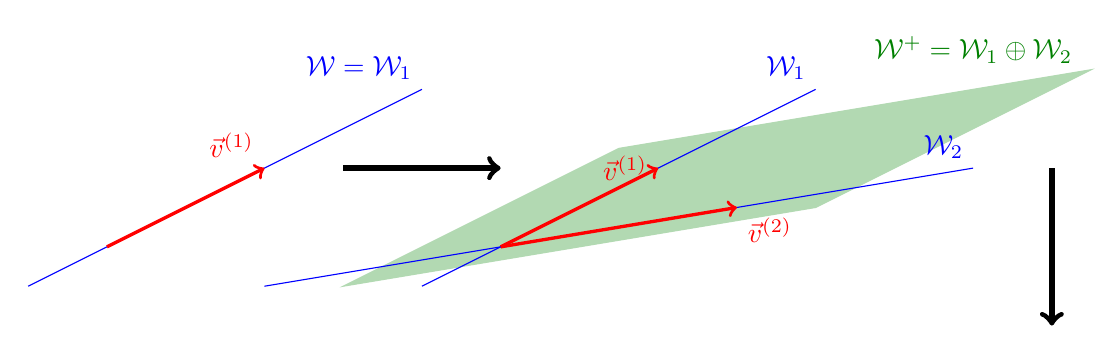
\begin{tikzpicture}
    \draw[blue] (-1,-0.5,0) -> (4,2,0) node[above left]{$\mathcal{W} = \mathcal{W}_1$};
    \draw[line width=1.2, red, ->] (0,0,0) -> (2,1,0) node[above left]{$\vec{v}^{(1)}$};
    \draw[line width=2, ->] (3,1,0) -- (5,1,0);
    \filldraw[Green!30] (3,-0.5,0) -- (6.5,1.25,0) -- (12.5,2.25,0) -- (9,0.5,0) -- cycle;
    \node[Green] at (11,2.5) {$\mathcal{W}^+ = \mathcal{W}_1 \oplus \mathcal{W}_2$};
    \draw[blue] (4,-0.5,0) -> (9,2,0) node[above left]{$\mathcal{W}_1$};
    \draw[line width=1.2, red, ->] (5,0,0) -> (7,1,0) node[left]{$\vec{v}^{(1)}$};
    \draw[blue] (2,-0.5,0) -> (11,1,0) node[above left]{$\mathcal{W}_2$};
    \draw[line width=1.2, red, ->] (5,0,0) -> (8,0.5,0) node[below right]{$\vec{v}^{(2)}$};
    \draw[line width=2, ->] (12,1,0) -- (12,-1,0);
    \end{tikzpicture}\\
    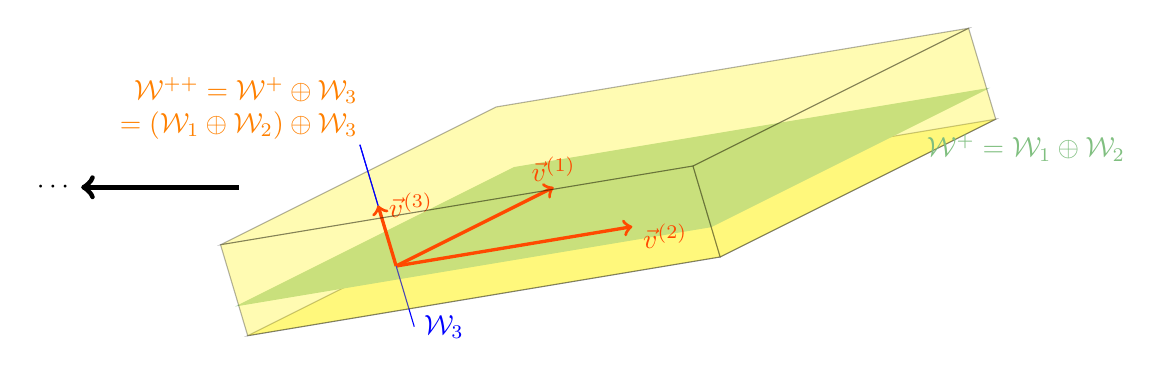
\begin{tikzpicture}
    \draw[black, fill=yellow, opacity=0.3] (3.5,-0.5,1) -- (7,1.25,1) -- (13,2.25,1) -- (9.5,0.5,1) -- cycle;
    \filldraw[Green!30] (3,-0.5,0) -- (6.5,1.25,0) -- (12.5,2.25,0) -- (9,0.5,0) -- cycle;
    \draw[line width=1.2, red, ->] (5,0,0) -> (7,1,0) node[above, yshift=-2]{$\vec{v}^{(1)}$};
    \draw[line width=1.2, red, ->] (5,0,0) -> (8,0.5,0) node[below right, yshift=5]{$\vec{v}^{(2)}$};
    \draw[blue] (3,0,-4) -> (6,0,2) node[right]{$\mathcal{W}_3$};
    \draw[line width=1.2, red, ->] (5,0,0) -> (4,0,-2) node[right]{$\vec{v}^{(3)}$};
    \draw[black, fill=yellow, opacity=0.3] (2,-0.5,-2) -- (5.5,1.25,-2) -- (11.5,2.25,-2) -- (8,0.5,-2) -- cycle;
    \draw[black, fill=yellow, opacity=0.3] (2,-0.5,-2) -- (3.5,-0.5,1) -- (9.5,0.5,1) -- (8,0.5,-2) -- cycle;
    \draw[black, fill=yellow, opacity=0.3] (11.5,2.25,-2) -- (13,2.25,1) -- (9.5,0.5,1) -- (8,0.5,-2) -- cycle;
    \node[Green!50] at (13,1.5) {$\mathcal{W}^+ = \mathcal{W}_1 \oplus \mathcal{W}_2$};
    \node[orange, align=right] at (3,2) {$\mathcal{W}^{++} = \mathcal{W}^+ \oplus \mathcal{W}_3$ \\
    $= (\mathcal{W}_1 \oplus \mathcal{W}_2) \oplus \mathcal{W}_3$};
    \draw[blue] (3,0,-4) -> (4,0,-2);
    \draw[line width=2, ->] (3,1,0) -- (1,1,0) node[left]{$\cdots$};
    \end{tikzpicture}
    \caption{Iteratively adding one-dimensional subspaces to the direct sum. Note that the lines, plane and "cuboid" all extend infinitely. We can only visualize up to a three-dimensional direct sum but it goes on even for higher dimensions.}
    \label{fig:directsumeachsubspace}
\end{figure}

%This also completes our previous proof mentioned in Definition \ref{inverseidentity}.
%\begin{thm}
%If $AP = A$, and $A$ is a invertible square matrix, then $P$ must be $I$.
%\paragraph{Proof}
%The assumption implies that $A$ has linearly independent column vectors. As a result, they cannot be expressed by other vectors. Consider any one of the column vector, like $\vec{u_i}$, then the linear system
%\begin{align*}
%A\vec{x} &= ([\vec{u_1}|\cdots|\vec{u_i}|\cdots|\vec{u_n}])\vec{x} = x_1\vec{u_1} + \cdots + x_i\vec{u_i} + \cdots + x_n\vec{u_n} \\
%&= \vec{u_i}
%\end{align*}
%will only have the solution
%\begin{align*}
%x_j &= 1 & \text{if $j = i$} \\
%x_j &= 0 & \text{if $j \neq i$}
%\end{align*}
%This means that $\vec{x} = \hat{e_i}$. Now if we expand $P = [\vec{p_1}|\cdots|\vec{p_i}|\cdots|\vec{p_n}]$, then we can write $AP = A$ as
%\begin{align*}
%AP &= [A\vec{p_1}|\cdots|A\vec{p_i}|\cdots|A\vec{p_n}] \\
%&= A = [\vec{u_1}|\cdots|\vec{u_i}|\cdots|\vec{u_n}]
%\end{align*}
%The readers are encouraged to verify the expression of $AP = [A\vec{p_1}|\cdots|A\vec{p_i}|\cdots|A\vec{p_n}]$ as a mental exercise, as from time to time we will partition such matrix product into columns. We have just found that for $A\vec{p_i} = \vec{u_i}$ to hold, $\vec{p_i}$ must be $\hat{e_i}$. This implies $P = [\hat{e_1}|...|\hat{e_i}|...|\hat{e_n}] = I$.
%\end{thm}

\section{The Four Fundamental Subspaces Induced by Matrices}

\subsection{Row Space, Column Space}

In Definition \ref{defn:colspace}, we have developed the notion of column space. For a $m\times n$ matrix $A = [\vec{v}^{(1)}|\vec{v}^{(2)}|\cdots|\vec{v}^{(n)}]$, its column space is the subspace generated by the $n$ $\mathbb{R}^m$ vectors $\vec{v}^{(j)}$, $j = 1,2,\ldots,n$. Similarly, we can also define the \index{Row Space}\keywordhl{row space} of a matrix. We formally define both of them below.

\begin{defn}[Column/Row Space]
\label{defn:colrowspace}
For an $m \times n$ real matrix $A$, its column space $\mathcal{C}(A)$ is the subspace spanned by its $n$ column vectors, $\vec{v}^{(1)}, \vec{v}^{(2)}, \ldots, \vec{v}^{(n)} \in \mathbb{R}^m$ as in $A = [\vec{v}^{(1)}|\vec{v}^{(2)}|\cdots|\vec{v}^{(n)}]$; Meanwhile its row space is the subspace spanned by its $m$ row vectors $\vec{w}^{(1)T}, \vec{w}^{(2)T}, \ldots, \vec{w}^{(m)T} \in \mathbb{R}^n$ as in
\begin{align*}
A = 
\left[\begin{array}{c}
\vec{w}^{(1)T} \\
\hline
\vec{w}^{(2)T} \\
\hline
\vdots \\
\hline
\vec{w}^{(m)T}
\end{array}\right]
\end{align*}
Notice that the row (column) space of a matrix is just the column (row) space of its transpos, hence we denote the row space of $A$ as $\mathcal{C}(A^T)$.
\end{defn}

For instance, in Example \ref{exmp:gentrimbasis}, the matrix
\begin{align*}
A &= 
\begin{bmatrix}
1 & 1 & 0 & -2\\
0 & -1 & 0 & 1\\
2 & 1 & 1 & 0\\
1 & -2 & 0 & 1
\end{bmatrix}
\end{align*}
actually has a column space of $\mathcal{C}(A) = \text{span}(\{(1,0,2,1)^T, (1,-1,1,-2)^T, \\ (0,0,1,0)^T, (-2,1,0,1)^T\}) = \text{span}(\{(1,0,2,1)^T, (1,-1,1,-2)^T, (0,0,1,0)^T\})$ of dimension $3$ despite the vectors are in $\mathbb{R}^4$. In middle of deriving this result we have produced the reduced row echelon form of $A$, which is 
\begin{align*}
\begin{bmatrix}
1 & 0 & 0 & -1\\
0 & 1 & 0 & -1\\
0 & 0 & 1 & 3\\
0 & 0 & 0 & 0 
\end{bmatrix}
\end{align*}
from which we can see the number of pivots, or \textit{rank}, is also $3$. In fact, just like the case above, the \index{Rank}\keywordhl{rank} of a matrix always indicates the dimension of its column space. This is due to Properties \ref{proper:findgenbasis} and \ref{proper:samenvecsbases}, leading to the following equivalent definition.
\begin{defn}[Rank]
\label{defn:rank}
The rank of a matrix $A$ is the number of leading 1s in its reduced row echelon form, which is also the amount of linearly independent vectors in any basis of its column space, i.e. the dimension of the column space.
\end{defn}
We can approach this from another angle, which involves restating previous results related to Gaussian Elimination. In Section \ref{section:linearind}, we have shown that elementary row operations preserve (the amount of) linear independent vectors, hence
\begin{proper}
\label{proper:elemrowopcolrank}
Elementary row operations does not change the number of dimensions in the column space of a matrix.
\end{proper}
The matrix $A$ will then have the same number of dimensions in its column space throughout the Gaussian Elimination procedure, which coincides with the number of linearly independent vectors and thus pivots in the final reduced row echelon form, establishing the equivalence in Definition \ref{defn:rank}. However, notice that elementary row operations do change the actual column space. On the other hand, for row space, we have an even stronger result.
\begin{proper}
\label{proper:elemrowoprowrank}
Elementary row operations does not change the row space of a matrix, and thus its dimension.
\end{proper}
which is not hard to accept. Swapping rows, and multiplying a row by some constant obviously does not affect the span of rows in the matrix. Adding to/subtracting from a row $R_p$ (also as a row vector $\vec{w}^{(p)T}$) by the constant multiple of another row $R_q$ ($\vec{w}^{(q)T}$) also will not alter it. To see this, observe that the newly resulted row vector is just a linear combination of the two input rows, i.e. the new $R_p$ becomes $\vec{w}^{(r)T} = \vec{w}^{(p)T} + c\vec{w}^{(q)T}$ (and hence $\vec{w}^{(p)T} = \vec{w}^{(r)T} - c\vec{w}^{(q)T}$). Using part (b) of Theorem \ref{thm:plusminus} twice, we have
\begin{align*}
&= \text{span}(\{\ldots, \vec{w}^{(p)}, \ldots, \vec{w}^{(q)}, \ldots, \vec{w}^{(r)}\}) \\
\mathcal{C}(A^T) &= \text{span}(\{\ldots, \vec{w}^{(p)}, \ldots, \vec{w}^{(q)}, \ldots\}) \\
&= \text{span}(\{\ldots, \vec{w}^{(r)}, \ldots, \vec{w}^{(q)}, \ldots\}) = \mathcal{C}(A'^T)
\end{align*}
where $A'$ denotes the matrix after the addition/subtraction elementary row operation. Our next key result relies on the observation that the dimensions of row and column space of a matrix in its reduced row echelon form are the same, or in other words,
\begin{proper}
\label{proper:rrefcolrowrank}
A matrix in reduced row echelon form has the same amount of (linearly independent) vectors in the basis of its row and column space.
\end{proper}
We will not read off the detailed arguments in the proof, but instead note that it is essentially an analysis of positions of the leading 1s and zeros in any reduced row echelon form. However, we will give an example to elucidate how it holds. Take a reduced row echelon form of
\begin{align*}
\begin{bmatrix}
1 & 1 & 0 & 0 & 1 \\
0 & 0 & 1 & 0 & 0 \\
0 & 0 & 0 & 1 & 1 \\
0 & 0 & 0 & 0 & 0 
\end{bmatrix}
\end{align*}
It is obvious that its column space is spanned by the basis $\{(1,0,0,0)^T, (0,1,0,0)^T, \\ (0,0,1,0)^T\}$, while a basis of its row space can be simply formed by the first three non-zero row vectors $\{(1,1,0,0,1), (0,0,1,0,0), (0,0,0,1,1)\}$. In this case, the dimension of row/column space of the reduced row echelon form is both $3$. With these observations, we can derive the desired result, sometimes referred to as \textit{"Column rank equals to row rank"}.
\begin{proper}
\label{proper:samecolrowrank}
For any matrix, the dimension of its column space is equal to that of its row space, i.e.
\begin{align*}
\dim(\mathcal{C}(A)) = \dim(\mathcal{C}(A^T))
\end{align*}
\end{proper}
\begin{proof}
Any matrix has a unique reduced row echelon form due to Theorem \ref{thm:uniquerref}, whose row/column space has the same number of dimensions by Properties \ref{proper:rrefcolrowrank}. According to Properties \ref{proper:elemrowopcolrank} and \ref{proper:elemrowoprowrank}, the elementary row operations done to convert the matrix to its reduced row echelon form leave both the dimensions of row and column space conserved, and thus the column rank and row rank in the starting matrix are equal.
\end{proof}
\begin{exmp}
\label{exmp:colrowspace}
Given a matrix
\begin{align*}
A = 
\begin{bmatrix}
1 & 1 & -2 & 1 \\
1 & 2 & 1 & -1 \\
1 & 0 & -5 & 3
\end{bmatrix}
\end{align*}
find a basis for its column/row space $\mathcal{C}(A)$ and $\mathcal{C}(A^T)$ and check if Properties \ref{proper:samecolrowrank} holds.
\end{exmp}
\begin{solution}
We first apply Gaussian Elimination to $A$, which leads to
\begin{align*}
\left[\begin{array}{@{\;}wc{10pt}wc{10pt}wc{10pt}wc{10pt}@{\;}}
1 & 1 & -2 & 1 \\
1 & 2 & 1 & -1 \\
1 & 0 & -5 & 3
\end{array}\right]
& \rightarrow
\left[\begin{array}{@{\;}wc{10pt}wc{10pt}wc{10pt}wc{10pt}@{\;}}
1 & 1 & -2 & 1 \\
0 & 1 & 3 & -2 \\
0 & -1 & -3 & 2
\end{array}\right]
& \begin{aligned}
R_2 - R_1 &\to R_2 \\
R_3 - R_1 &\to R_3
\end{aligned} \\
& \rightarrow
\left[\begin{array}{@{\;}wc{10pt}wc{10pt}wc{10pt}wc{10pt}@{\;}}
1 & 1 & -2 & 1 \\
0 & 1 & 3 & -2 \\
0 & 0 & 0 & 0
\end{array}\right]
& R_3 - R_2 \to R_3 \\
& \rightarrow
\left[\begin{array}{@{\;}wc{10pt}wc{10pt}wc{10pt}wc{10pt}@{\;}}
1 & 0 & -5 & 3 \\
0 & 1 & 3 & -2 \\
0 & 0 & 0 & 0
\end{array}\right]
& R_1 - R_2 \to R_1
\end{align*}
The number of pivotal columns is $2$, and from the reduced row echelon form we obtain the dependence relations where the first two column vectors $(1,1,1)^T$ and $(1,2,0)^T$ are linearly independent while the last two column vectors $(-2,1,-5)^T = -5(1,1,1)^T + 3(1,2,0)^T$ and $(1,-1,3)^T = 3(1,1,1)^T - 2(1,2,0)^T$ are linear combinations of the previous two. Hence $\mathcal{C}(A)$ has a basis of $\{(1,1,1)^T, (1,2,0)^T\}$ and $\dim(\mathcal{C}(A)) = 2$. On the other hand, to find the row space we consider $A^T$ and repeat the elimination process again as follows. However, notice that according to the dependence relations for the column vectors in $A$ above, we can immediately do the corresponding addition/subtraction operations for the rows in $A^T$, to reduce the third/fourth rows, obtaining
\begin{align*}
\left[\begin{array}{@{\;}wc{10pt}wc{10pt}wc{10pt}wc{10pt}@{\;}}
1 & 1 & 1 \\
1 & 2 & 0 \\
-2 & 1 & -5 \\
1 & -1 & 3
\end{array}\right] 
&\rightarrow
\left[\begin{array}{@{\;}wc{10pt}wc{10pt}wc{10pt}wc{10pt}@{\;}}
1 & 1 & 1 \\
1 & 2 & 0 \\
0 & 0 & 0 \\
0 & 0 & 0
\end{array}\right] 
& \begin{aligned}
R_3 + 5R_1 - 3R_2 &\to R_3, \\
R_4 - 3R_1 + 2R_2 &\to R_4
\end{aligned}
\end{align*}
and the next step is straight-forward:
\begin{align*}
\left[\begin{array}{@{\;}wc{10pt}wc{10pt}wc{10pt}wc{10pt}@{\;}}
1 & 1 & 1 \\
1 & 2 & 0 \\
0 & 0 & 0 \\
0 & 0 & 0
\end{array}\right] 
&\rightarrow
\left[\begin{array}{@{\;}wc{10pt}wc{10pt}wc{10pt}wc{10pt}@{\;}}
1 & 1 & 1 \\
0 & 1 & -1 \\
0 & 0 & 0 \\
0 & 0 & 0
\end{array}\right] 
& R_2 - R_1 \to R_2 \\
&\rightarrow
\left[\begin{array}{@{\;}wc{10pt}wc{10pt}wc{10pt}wc{10pt}@{\;}}
1 & 0 & 2 \\
0 & 1 & -1 \\
0 & 0 & 0 \\
0 & 0 & 0
\end{array}\right] 
& R_1 - R_2 \to R_1
\end{align*}
which reveals that the first two columns (representing the first two row vectors in $A$) are linearly independent and the third column (the last row vector in $A$) is redundant ($(1,0,-5,3)^T = 2(1,1,-2,1)^T-(1,2,1,-1)^T$). Therefore $\mathcal{C}(A^T)$ has a basis of $\{(1,1,-2,1)^T, (1,2,1,-1)^T\}$, and $\dim(\mathcal{C}(A^T)) = 2 = \dim(\mathcal{C}(A))$, and Properties \ref{proper:samecolrowrank} is true in this case.
\end{solution}
Finally, in view of Definitions \ref{defn:span} and \ref{defn:colrowspace}, the analysis about solving linear systems in Section \ref{section:SolveLinSys} can be summarized as
\begin{proper}
A linear system $A\vec{x} = \vec{h}$ is consistent if and only if $\vec{h}$ is in the column space of $A$.
\end{proper}

\subsection{Null Space, Rank-Nullity Theorem}
\label{section:null}

As we have briefly mentioned in the end of last chapter, the solution of a linear system $A\vec{x} = \vec{h}$, where $A$ is an $m \times n$ matrix and $\vec{x} \in \mathbb{R}^n$, can be viewed as some sort of a solution space. In Section \ref{subsection:SolLinSysGauss} we know that it is made up of the particular and complementary solution, where the latter corresponding to the family of $\vec{x} = \vec{x}_0$ ($= \vec{x}_c$ using the notation in that section) that satisfies the homogeneous part $A\vec{x} = \textbf{0}$. The set $\vec{x}_0 \in \mathbb{R}^n$ can be shown to form a subspace of $\mathbb{R}^n$\footnote{To show this we check the two conditions in Theorem \ref{thm:subspacecriteria}. Let $\vec{x}_0^{(1)}$ and $\vec{x}_0^{(2)}$ be two vectors in the null space $\vec{x}_0$. Then we have: 1. $A(\vec{x}_0^{(1)} + \vec{x}_0^{(2)}) = A\vec{x}_0^{(1)} + A\vec{x}_0^{(2)} = \textbf{0} + \textbf{0} = \textbf{0}$, so $\vec{x}_0^{(1)} + \vec{x}_0^{(2)} \in \vec{x}_0$, and 2. $A(a\vec{x}_0^{(1)}) = a(A\vec{x}_0^{(1)}) = a\textbf{0} = \textbf{0}$, hence $a\vec{x}_0^{(1)} \in \vec{x}_0$.}, and this subspace is then called the \index{Null Space}\keywordhl{null space} of $A$.
\begin{defn}[Null Space]
\label{defn:nullspace}
For an $m \times n$ real matrix $A$, its null space $\mathcal{N}(A)$ is the subspace consisted of all solution vectors $\vec{x} = \vec{x}_0 \in \mathbb{R}^n$ to the matrix equation $A\vec{x} = \textbf{0}$. The dimension of null space is called \index{Nullity}\keywordhl{nullity}.
\end{defn}
This definition of nullity as the dimension of null space is consistent with that in Section \ref{subsection:SolLinSysGauss} where nullity is initially given by the number of columns in the matrix minus the amount of leading 1s (rank) in its rref, or equivalently the number of non-pivotal columns. To see this, observe that any solution $\vec{x}_0$ to $A\vec{x} = \textbf{0}$ is also the solution to $A_{\text{rref}}\vec{x} = \textbf{0}$ and vice versa, via elementary matrices. Hence the null space and nullity of $A$ will be the same as that of $A_{\text{rref}}$. Previously we have assigned free variables to the non-pivotal columns (let's say there is $k$ of them) of $A_{\text{rref}}$ and derive $\vec{x}_0$ where they are generated by $k$ pairs of free variables and column vectors ($\vec{x}_0^{(1)}, \vec{x}_0^{(2)}, \ldots, \vec{x}_0^{(k)}$). It is clear that such a procedure will ensure these $k$ vectors are linearly independent as each of them has a component of $1$ in the position corresponding to that particular free variable indicated by the rref and $0$s in other positions corresponding to other free variables (see Example \ref{exmp:underdetsys} for an instance). We claim that they also span the entire null space of $A_{\text{rref}}$.\footnote{Assume the contrary so that the span of $\{\vec{x}_0^{(1)}, \vec{x}_0^{(2)}, \ldots, \vec{x}_0^{(k)}\}$ does not cover the whole null space, then the dimension of null space has to be greater than $k$ by Properties $\ref{proper:dimWleqV}$. Without loss of generality, let the "correct" dimension of null space to be $k+1$. Then by (c) of Properties \ref{proper:linindspanbasisnewver}, there exists $\vec{x}_0^{(k+1)}$ such that $\{\vec{x}_0^{(1)}, \vec{x}_0^{(2)}, \ldots, \vec{x}_0^{(k)}, \vec{x}_0^{(k+1)}\}$ are basis of the null space. This $\vec{x}_0^{(k+1)}$ can be made to take the value of $0$ at all $k$ positions where the free variables reside by subtracting it by appropriate multiples of $\vec{x}_0^{(j)}$, $j \neq k+1$, without altering the null space (c.f.\ Footnote \ref{foot:ft14}), and by doing so non-zero components of $\vec{x}_0^{(k+1)}$ only appear in positions corresponding to leading 1s in $A_{\text{rref}}$. This causes a contradiction since $A_{\text{rref}}\vec{x}_0^{(k+1)} = \textbf{0}$ then implies that there exists a non-trivial dependence relation between the pivotal column vectors themselves.} Hence by the definition given in Section \ref{section:subspacebasis} they form a basis for the null space of $A_{\text{rref}}$ as well as $A$ and by Properties \ref{proper:samenvecsbases} the dimension of null space of $A$ is also $k$.

Using Definitions \ref{defn:colrowspace}, \ref{defn:rank}, and \ref{defn:nullspace} to rephrase, the preceding discussion means that the rank of a matrix plus its nullity equals to its number of columns, which leads to the so-called \index{Rank-nullity Theorem}\keywordhl{Rank-nullity Theorem}.
\begin{thm}[Rank-nullity Theorem]
\label{thm:ranknullity}
For a real $m \times n$ matrix $A$, we have
\begin{align*}
\dim(\mathcal{C}(A)) + \dim(\mathcal{N}(A)) &= \text{rank}(A) + \text{nullity}(A) = n \\
&= \dim(\mathcal{C}(A^T)) + \dim(\mathcal{N}(A))
\end{align*}
where $\dim(\mathcal{C}(A)) = \dim(\mathcal{C}(A^T)) = \text{rank}(A)$ by Properties \ref{proper:samecolrowrank}.
\end{thm}
An invertible square matrix has a reduced row echelon form of an identity matrix according to Theorem \ref{thm:equiv3}, and since an identity matrix has \textit{full rank}\footnote{An $m \times n$ matrix $A$ is said to have full rank if $\text{rank}(A) = \text{min}(m,n)$} (Definition \ref{defn:rank}), by the Rank-nullity Theorem \ref{thm:ranknullity} above, we have
\begin{proper}
A $n \times n$ square matrix is invertible if and only if its rank and nullity are $n$ and $0$. 
\end{proper}

A notable relationship between row space and null space is that any pair of two vectors coming from the respective subspaces will be orthogonal to each other. 
\begin{proper}
\label{proper:rownullortho}
Given a real matrix $A$, any vector in its row space $\mathcal{C}(A^T)$ is orthogonal to all vectors in its null space $\mathcal{N}(A)$ and vice versa.
\end{proper}
\begin{proof}
Let the shape of $A$ be $m \times n$, we can express $A$ in the form of its row vectors as
\begin{align*}
A = 
\left[\begin{array}{c}
\vec{w}^{(1)T} \\
\hline
\vec{w}^{(2)T}\\
\hline
\vdots \\
\hline
\vec{w}^{(m)T}
\end{array}\right]
\end{align*}
and the corresponding homogeneous system $A\vec{x} = \textbf{0}$ then can be written as
\begin{align*}
A\vec{x} =
\left[\begin{array}{c}
\vec{w}^{(1)T} \\
\hline
\vec{w}^{(2)T}\\
\hline
\vdots \\
\hline
\vec{w}^{(m)T}
\end{array}\right]
\vec{x}
=
\left[\begin{array}{c}
\vec{w}^{(1)T} \cdot \vec{x} \\
\vec{w}^{(2)T} \cdot \vec{x} \\
\vdots \\
\vec{w}^{(m)T} \cdot \vec{x}
\end{array}\right]
= \textbf{0}
=
\left[\begin{array}{c}
0 \\
0 \\
\vdots \\
0
\end{array}\right]
\end{align*}
where for a solution $\vec{x} = \vec{x}_0$ in the null space of $A$, each of the dot products $\vec{w}^{(i)T} \cdot \vec{x}_0 = 0$, $i = 1, 2, \ldots, m$, has to be equal to zero. Any vector in the row space of $A$ can be expressed as $\vec{w} = c_1\vec{w}^{(1)} + c_2\vec{w}^{(2)} + \cdots + c_m\vec{w}^{(m)}$ by Definitions \ref{defn:colrowspace} and \ref{defn:span}, and subsequently, its dot product with $\vec{x}_0$
\begin{align*}
\vec{w}^T \cdot \vec{x}_0 &= (c_1\vec{w}^{(1)} + c_2\vec{w}^{(2)} + \cdots + c_m\vec{w}^{(m)})^T \cdot \vec{x}_0 \\
&= c_1(\vec{w}^{(1)T} \cdot \vec{x}_0) + c_2(\vec{w}^{(2)T} \cdot \vec{x}_0) + \cdots + c_m(\vec{w}^{(m)T} \cdot \vec{x}_0) \\
&= c_1(0) + c_2(0) + \cdots + c_m(0) = 0
\end{align*}
is also zero, therefore they are orthogonal by Properties \ref{proper:dotorth}, which implies that any vector in $\mathcal{C}(A^T)$ is orthogonal to any another vector in $\mathcal{N}(A)$.
\end{proof}
As a corollary, this is equivalent to all vectors in the generating set or basis for the row space for a matrix being orthogonal to all vectors in those for its null space. The following additional observation will be useful later.
\begin{proper}
\label{proper:ortholinind}
Non-zero orthogonal vectors are linearly independent.
\end{proper}
\begin{proof}
We will only prove the case with two vectors in $\mathbb{R}^n$ but those with multiple vectors can be derived in the same essence. Consider $c_1\vec{u}^{(1)} + c_2\vec{u}^{(2)} = \textbf{0}$ where $\vec{u}^{(1)}$ and $\vec{u}^{(2)}$ are orthogonal, i.e. $\vec{u}^{(1)} \cdot \vec{u}^{(2)} = 0$. Taking dot product with $\vec{u}_1$ on both sides gives
\begin{align*}
\vec{u}^{(1)} \cdot (c_1\vec{u}^{(1)} + c_2\vec{u}^{(2)}) = c_1(\vec{u}^{(1)} \cdot \vec{u}^{(1)}) + c_2(\vec{u}^{(1)} \cdot \vec{u}^{(2)}) &= \vec{u}^{(1)} \cdot \textbf{0} \\
c_1 \norm{\vec{u}^{(1)}}^2 + c_2 (0) = c_1 \norm{\vec{u}^{(1)}}^2 &= 0
\end{align*}
Since $\vec{u}_1$ is non-zero, $\norm{\vec{u}_1}^2 > 0$, and $c_1$ must be zero. In a similar vein, we can show that $c_2$ is zero as well. Therefore the only solution to the equation $c_1\vec{u}_1 + c_2\vec{u}_2 = \textbf{0}$ is the trivial solution $c_1 = c_2 = 0$. By Theorem \ref{thm:linearindep}, the two vectors are linearly independent.
\end{proof}
\begin{exmp}
\label{exmp:colrowspace2}
For the matrix in Example \ref{exmp:colrowspace}, find its null space and check if Properties \ref{proper:rownullortho} and Theorem \ref{thm:ranknullity} hold.
\end{exmp}
\begin{solution}
The homogeneous system corresponding to the matrix is
\begin{align*}
\left[\begin{array}{@{\;}wc{10pt}wc{10pt}wc{10pt}wc{10pt}|wc{10pt}@{\;}}
1 & 1 & -2 & 1 & 0\\
1 & 2 & 1 & -1 & 0\\
1 & 0 & -5 & 3 & 0
\end{array}\right]
\end{align*}
which can be reduced, following the same steps in Example \ref{exmp:colrowspace}, to
\begin{align*}
\left[\begin{array}{@{\;}wc{10pt}wc{10pt}wc{10pt}wc{10pt}|wc{10pt}@{\;}}
1 & 0 & -5 & 3 & 0 \\
0 & 1 & 3 & -2 & 0\\
0 & 0 & 0 & 0 & 0
\end{array}\right]
\end{align*}
where there are two non-pivotal columns and hence two free parameters can be assigned to them. Let $x_3 = s$ and $x_4 = t$, then $x_1 = 5s - 3t$ and $x_2 = -3s + 2t$. So the solution to the system is
\begin{align*}
\begin{bmatrix}
x_1 \\
x_2 \\
x_3 \\
x_4
\end{bmatrix}
=
\begin{bmatrix}
5s-3t \\
-3s+2t \\
s \\
t
\end{bmatrix}
=
s
\begin{bmatrix}
5\\
-3\\
1\\
0
\end{bmatrix}
+ t
\begin{bmatrix}
-3 \\
2 \\
0 \\
1
\end{bmatrix}
\end{align*}
and thus a basis for the null space is $\{(5,-3,1,0)^T, (-3,2,0,1)^T\}$ where these two vectors are clearly linearly independent (by observing the $0$ and $1$ of the last two components). As found in Example \ref{exmp:colrowspace}, the basis for its row space is $\{(1,1,-2,1)^T, (1,2,1,-1)^T\}$. Subsequently, checking orthogonality between the two bases is straight-forward, and we will only do this for the first vector in the row space basis against the null space basis.
\begin{align*}
(5,-3,1,0)^T \cdot (1,1,-2,1)^T &= (5)(1)+(-3)(1)+(1)(-2)+(0)(1) = 0 \\
(-3,2,0,1)^T \cdot (1,1,-2,1)^T &= (-3)(1)+(2)(1)+(0)(-2)+(1)(1) = 0
\end{align*}
Furthermore, the dimension of null space, or the nullity, is $\dim{\mathcal{N}(A)} = 2$. Previously we have also found that $\dim{\mathcal{C}(A)} = \text{rank}(A) = 2$. So $\text{rank}(A) + \text{nullity}(A) = 2+2 = 4$, and Theorem \ref{thm:ranknullity} is true.
\end{solution}
Short Exercise: Show that \footnote{Replace $A$ by $A^T$ in Theorem \ref{thm:ranknullity} to get $\dim(\mathcal{C}(A^T)) + \dim(\mathcal{N}(A^T)) = m$.}
\begin{align*}
\dim(\mathcal{C}(A^T)) + \dim(\mathcal{N}(A^T)) = \dim(\mathcal{C}(A)) + \dim(\mathcal{N}(A^T)) = m   
\end{align*} $\mathcal{N}(A^T)$ is also known as the \index{Left Null Space}\keywordhl{left null space} of $A$.

By Properties \ref{proper:rownullortho} and \ref{proper:ortholinind}, vectors in the row space and null space of an $m \times n$ matrix $A$ are linearly independent of each other and can form a direct sum $\mathcal{C}(A^T) \oplus \mathcal{N}(A)$ according to Definition \ref{defn:directsum}. Note that they are the complement to each other with respect to this direct sum according to Properties \ref{proper:complement}. Since $\mathcal{C}(A^T) \subseteq \mathbb{R}^n$, $\mathcal{N}(A) \subseteq \mathbb{R}^n$ and hence $\mathcal{C}(A^T) \oplus \mathcal{N}(A) \subseteq \mathbb{R}^n$, from Theorem \ref{thm:ranknullity} and Properties \ref{proper:dimWleqV}, we conclude that $\mathcal{C}(A^T) \oplus \mathcal{N}(A)$ which has a dimension of $n$, is just $\mathbb{R}^n$. In other words, the row space and null space of a matrix can reconstruct the real $n$-space by forming their direct sum. The similar can be said for its column and left null space. Furthermore, since all vectors in the row space (column space) are orthogonal to those in the (left) null space (and vice versa) via Properties \ref{proper:rownullortho}, we say that they are actually an \index{Orthogonal Complement}\keywordhl{orthogonal complement} to each other.

\begin{proper}
\label{proper:funsubsortho}
For a real $m \times n$ matrix $A$, we have
\begin{align*}
& \mathcal{C}(A^T) \oplus \mathcal{N}(A) = \mathbb{R}^n & & \mathcal{C}(A) \oplus \mathcal{N}(A^T) = \mathbb{R}^m
\end{align*}
where $\mathcal{C}(A^T)^\perp = \mathcal{N}(A)$, $\mathcal{N}(A)^\perp = \mathcal{C}(A^T)$, and $\mathcal{C}(A)^\perp = \mathcal{N}(A^T)$, $\mathcal{N}(A^T)^\perp = \mathcal{C}(A)$, with $^\perp$ denoting an orthogonal complement.
\end{proper}

We conclude the relationships between the column, row, null, and left null space, a.k.a the \index{The Four Fundamental Subspaces}\keywordhl{Four fundamental subspaces} induced by a matrix, with a diagram (Figure \ref{fig:foursubspaces}). \par
\begin{figure}
    \centering
    \begin{tikzpicture}[>={Stealth[length=5pt]}]
    \node[opacity=0.1,scale=5] at (0,0) {$\mathbb{R}^n$}; 
    \node[opacity=0.1,scale=5] at (8,0) {$\mathbb{R}^m$};
    \draw[SkyBlue] (0,0) -- (2,2.8) -- (-0.1,4.3) -- (-2.1,1.5) -- cycle; 
    \node[align=left, scale=0.7] at (0,2.3) {Row space \\ $\mathcal{C}(A^T)$};
    \draw[SkyBlue] (0,0) -- (-1, -1.4) -- (1.8,-3.4) -- (2.8,-2) -- cycle;
    \node[align=left, scale=0.7] at (0.9,-1.7) {Null space \\ $\mathcal{N}(A)$};
    \draw (0.2, 0.28) -- (0.48, 0.08) -- (0.28, -0.2);
    \node at (0,5) {$\dim = r$};
    \node at (-1,-3) {$\dim = n-r$};
    \draw[CarnationPink] (8,0) -- (6,2.8) -- (8.1,4.3) -- (10.1,1.5) -- cycle;
    \node[align=left,scale=0.7] at (8.1,2) {Column space \\ $\mathcal{C}(A)$};
    \draw[CarnationPink] (8,0) -- (8.8,-8/7) -- (4.8,-2.8-8/7) -- (4,-2.8) -- cycle;
    \node[align=left,scale=0.7] at (6.6,-2) {Left null space \\ $\mathcal{N}(A^T)$};
    \draw (7.8, 0.28) -- (7.52, 0.08) -- (7.72, -0.2);
    \node at (6.5,4.5) {$\dim = r$};
    \node at (9,-2.5) {$\dim = m-r$};
    \node[scale=2.5, opacity=0.5] at (3.5,4) {$A_{m \times n}$};
    \node[circle,fill,inner sep=2pt,Green] at (0,0) {};
    \node at (-0.5,0) {$\textbf{0}$};
    \node[circle,fill,inner sep=2pt,yellow] at (8,0) {};
    \node at (8.5,0) {$\textbf{0}$};
    \draw[->] (1,0.5) -- (7,2.5) node[sloped, midway, below]{$A\vec{x} = \vec{h}$};
    \draw[dashed, -{Circle}] (1,0.5) -- (-0.4,1.5) node[left]{$\vec{x}_r$};
    \draw[dashed, -{Circle}] (1,0.5) -- (-0.2,-1.18) node[below]{$\vec{x}_n$};
    \node[circle,fill,inner sep=2pt] at (1,0.5) {};
    \node at (1,0.5) [below right]{$\vec{x} = \vec{x}_r + \vec{x}_n$};
    \draw[dashed, ->] (-0.2,-1.18) -- (8,0) node[sloped, pos=0.7, above]{$A\vec{x}_n = \textbf{0}$};
    \draw[dashed, ->] (-0.4,1.5) -- (7,2.5) node[sloped, midway, above]{$A\vec{x}_r = \vec{h}$};
    \node[above] at (7,2.6) {$\vec{h}$};
    \end{tikzpicture}
    \caption{The relationships between the four fundamental subspaces for an $m \times n$ real matrix $A$ of rank $r$: the row space $\mathcal{C}(A^T)$, null space $\mathcal{N}(A)$, column space $\mathcal{C}(A)$, left null space $\mathcal{N}(A^T)$. Any vector $\vec{x} \in \mathbb{R}^n$ can be partitioned into $\vec{x} = \vec{x}_r + \vec{x}_n$ uniquely, where $\vec{x}_r \in \mathcal{C}(A^T) \subseteq \mathbb{R}^n$ and $\vec{x}_n \in \mathcal{N}(A) \subseteq \mathbb{R}^n$ are in the row/null space of $A$ respectively. The matrix $A$ maps $\vec{x}_n$ to the zero vector in $\mathbb{R}^m$ and $\vec{x}_r$ to some vector $\vec{h} \in \mathcal{C}(A) \subseteq \mathbb{R}^m$ in the column space of $A$. The total effect on $\vec{x}$ multiplied by $A$, is the sum of the two responses: $A\vec{x} = A(\vec{x}_r + \vec{x}_n) = A\vec{x}_r + A\vec{x}_n = \vec{h} + \textbf{0} = \vec{h}$.}
    \label{fig:foursubspaces}
\end{figure}

Last but not least, we end this chapter with a useful result.
\begin{proper}
\label{proper:rankABsmaller}
For two (real) $m \times r$ and $r \times n$ matrices $A$ and $B$, the rank of $AB$
\begin{align*}
\text{rank}(AB) \leq \min(\text{rank}(A),\text{rank}(B))
\end{align*}
is capped by the smaller of ranks of $A$ and $B$.
\end{proper}
\begin{proof}
The column space of $AB$ is a subset of that of $A$, i.e.\ $\mathcal{C}(AB) \subseteq \mathcal{C}(A)$, because the columns of $AB$ can be viewed as
\begin{align*}
AB &= \begin{bmatrix}
A_1|A_2|\cdots|A_r
\end{bmatrix}
\begin{bmatrix}
b_{11} & b_{12} & \cdots & b_{1n} \\
b_{21} & b_{22} & & b_{2n} \\
\vdots & & \ddots & \vdots \\
b_{r1} & b_{r2} & \cdots & b_{rn}
\end{bmatrix} \\
&= \begin{bmatrix}
b_{11}A_1 + b_{21}A_2 + \cdots + b_{r1}A_r|\cdots|b_{1n}A_1 + b_{2n}A_2 + \cdots + b_{rn}A_r
\end{bmatrix}
\end{align*}
(similar to the explanation for the CR Factorization, where $A_j$ is the $j$-th column of $A$) which shows that the columns of $AB$ are linear combinations of columns in $A$ and hence are in the column space of $A$. By Properties \ref{proper:WcontainsspanS}, the column space of $A$ then contains the column space of $AB$. Applying Properties \ref{proper:dimWleqV} we have $\text{rank}(AB) = \dim(\mathcal{C}(AB)) \leq \dim(\mathcal{C}(A)) = \text{rank}(A)$. The same argument on the row space of $AB$ and $B$ similarly shows that $\text{rank}(AB) \leq \text{rank}(B)$ and the desired inequality follows.
\end{proof}
Short Exercise: Show that $\text{rank}(AB) = \text{rank}(A)$ if $B$ is an invertible square matrix.\footnote{$\text{rank}(A) = \text{rank}(ABB^{-1}) \leq \text{rank}(AB) \leq \text{rank}(A)$ by applying Properties \ref{proper:rankABsmaller} twice. So $\text{rank}(AB)$ is "sandwiched" by and must be equal to $\text{rank}(A)$.}

\section{Python Programming}
To check linear independence and find a basis for columns in a matrix (or in general, any basis from a spanning set), we can use the \verb|columnspace| method in \verb|sympy|. Let's test it with the matrix in Example \ref{exmp:colrowspace}.
\begin{lstlisting}
import sympy

myMatrix = sympy.Matrix([[1., 1., -2., 1.],
                         [1., 2., 1., -1.],
                         [1., 0., -5., 3.]])
print(myMatrix.columnspace())
\end{lstlisting}
which gives
\begin{lstlisting}
[Matrix([        
[1.0],
[1.0],
[1.0]]), 
Matrix([
[1.0],
[2.0],
[  0]])]   
\end{lstlisting}
as expected. The rank can be found in two ways.
\begin{lstlisting}
print(myMatrix.rank()) # or len(myMatrix.columnspace())
\end{lstlisting}
This returns \verb|2| correctly. We can make a basis for the row space similarly by the \verb|rowspace| method. In the same manner, the null space is computed by the \verb|nullspace| method:
\begin{lstlisting}
print(myMatrix.nullspace())
\end{lstlisting}
producing an output of
\begin{lstlisting}
[Matrix([
[ 5.0],
[-3.0],
[   1],
[   0]]), 
Matrix([
[-3.0],
[ 2.0],
[   0],
[   1]])]
\end{lstlisting}
The nullity is then simply calculated by \verb|len(myMatrix.nullspace())|, which gives a right answer of \verb|2|. Finally, CR Factorization is computed via the \verb|rank_decomposition| method, where
\begin{lstlisting}
C, R = myMatrix.rank_decomposition()
print(C, R)    
\end{lstlisting}
gives
\begin{lstlisting}
Matrix([[1.00, 1.00], 
        [1.00, 2.00], 
        [1.00, 0]])
Matrix([[1, 0, -5.00, 3.00], 
        [0, 1, 3.00, -2.00]])        
\end{lstlisting}
where the matrix $C$ is essentially the same as that comes from \verb|columnspace|.

\section{Exercises}

\begin{Exercise}
For $\vec{v}^{(1)} =
\begin{bmatrix}
1\\
1\\
0
\end{bmatrix}$,
$\vec{v}^{(2)} =
\begin{bmatrix}
1\\
0\\
1
\end{bmatrix}$,
$\vec{v}^{(3)} =
\begin{bmatrix}
0\\
1\\
1
\end{bmatrix}$,
find the constants $a$, $b$, $c$ such that their linear combination $a\vec{v}^{(1)} + b\vec{v}^{(2)} + c\vec{v}^{(3}$ equals to 
\begin{enumerate}[label=(\alph*)]
\item $(3,2,9)^T$, 
\item $(9,1,5)^T$.
\end{enumerate}
\end{Exercise}

\begin{Exercise}
Determine if the following sets of vectors are linearly independent.
\begin{enumerate}[label=(\alph*)]
\item $\vec{u} = (2,-1)^T$, $\vec{v} = (-4,2)^T$,
\item $\vec{u} = (1,2,3)^T$, $\vec{v} = (6,7,9)^T$, $\vec{w} = (4,8,5)^T$, and
\item $\vec{u} = (1,3,3)^T$, $\vec{v}=(3,2,9)^T$, $\vec{w} = (1,-4,3)^T$.
\end{enumerate}
\end{Exercise}

\begin{Exercise}
Given a spanning set $\mathcal{G} = \{\vec{v}^{(1)}, \vec{v}^{(2)}, \vec{v}^{(3)}, \vec{v}^{(4)}\}$ in which $\vec{v}^{(1)} = (1,3,0,1)^T$, $\vec{v}^{(2)} = (1,-1,2,-1)^T$, $\vec{v}^{(3)} = (-1,2,1,2)^T$, $\vec{v}^{(4)} = (3,0,1,-2)^T$, determine if 
\begin{enumerate}[label=(\alph*)]
\item $(1,4,3,2)^T$, and
\item $(1,2,-3,1)^T$.
\end{enumerate}
are in the subspace generated by $\mathcal{G}$.
\end{Exercise}

\begin{Exercise}
For the basis $\mathcal{B} = \{\vec{v}^{(1)}, \vec{v}^{(2)}, \vec{v}^{(3)}\}$, where $\vec{v}^{(1)} = (6,1,2)^T$,
$\vec{v}^{(2)} = (1,0,1)^T$,
$\vec{v}^{(3)} = (2,3,3)^T$
(relative to the standard basis $\mathcal{S}$), do the following coordinate conversion.
\begin{enumerate}[label=(\alph*)]
\item Find the coordinates of $(5, 2, 3)^T$ in the $\mathcal{B}$ frame,
\item Transform $(1, -1, 1)^T_B$ from the $\mathcal{B}$ system back to the the standard basis $\mathcal{S}$.
\end{enumerate}
\end{Exercise}

\begin{Exercise}
Show that $\mathcal{B} = \{\vec{w}^{(1)}, \vec{w}^{(2)}, \vec{w}^{(3)}\}$, where $\vec{w}^{(1)} = (1,-1,0,1)^T$,
$\vec{w}^{(2)} = (2,1,1,0)^T$,
$\vec{w}^{(3)} = (1,2,-1,1)^T$ forms a basis for the subspace generated by itself, and find the coordinates of $\vec{v} = (1.-1,-2,3)^T$ with respect to this basis.
\end{Exercise}

\begin{Exercise}
Prove that for any two subspaces $\mathcal{W}_1, \mathcal{W}_2 \subseteq \mathcal{V}$. Their intersection $\mathcal{W}_1 \cap \mathcal{W}_2$ is also a subspace of $\mathcal{V}$. How about their union?
\end{Exercise}

\begin{Exercise}
Show that $\mathcal{W}_1 = \text{span}(\{(1,0,0,1)^T, (0,1,-1,1)^T\})$ and $\mathcal{W}_2 = \text{span}(\{(1,0,1,-1)^T\})$ can be composed to produce a direct sum $\mathcal{W}_1 \oplus \mathcal{W}_2$. Find bases for $\mathcal{W}_1$, $\mathcal{W}_2$ and hence this direct sum. Express $(2,0,1,0)^T$ in the direct sum basis as the combined coordinates of the two smaller subspaces.
\end{Exercise}

\begin{Exercise}
Find (bases for) the column, row, null and left null space of 
\begin{align*}
A = 
\begin{bmatrix}
1 & 0 & 1 & 1 \\
0 & 1 & -1 & 1 \\
1 & 2 & -1 & 0 \\
1 & 0 & 1 & 0
\end{bmatrix}
\end{align*}
and check if Theorem \ref{thm:ranknullity} and Properties \ref{proper:funsubsortho} hold in this case.
\end{Exercise}